\subsection{External Interfaces}
\subsubsection{User Interfaces}

\begin{figure}[H]
    \centering
    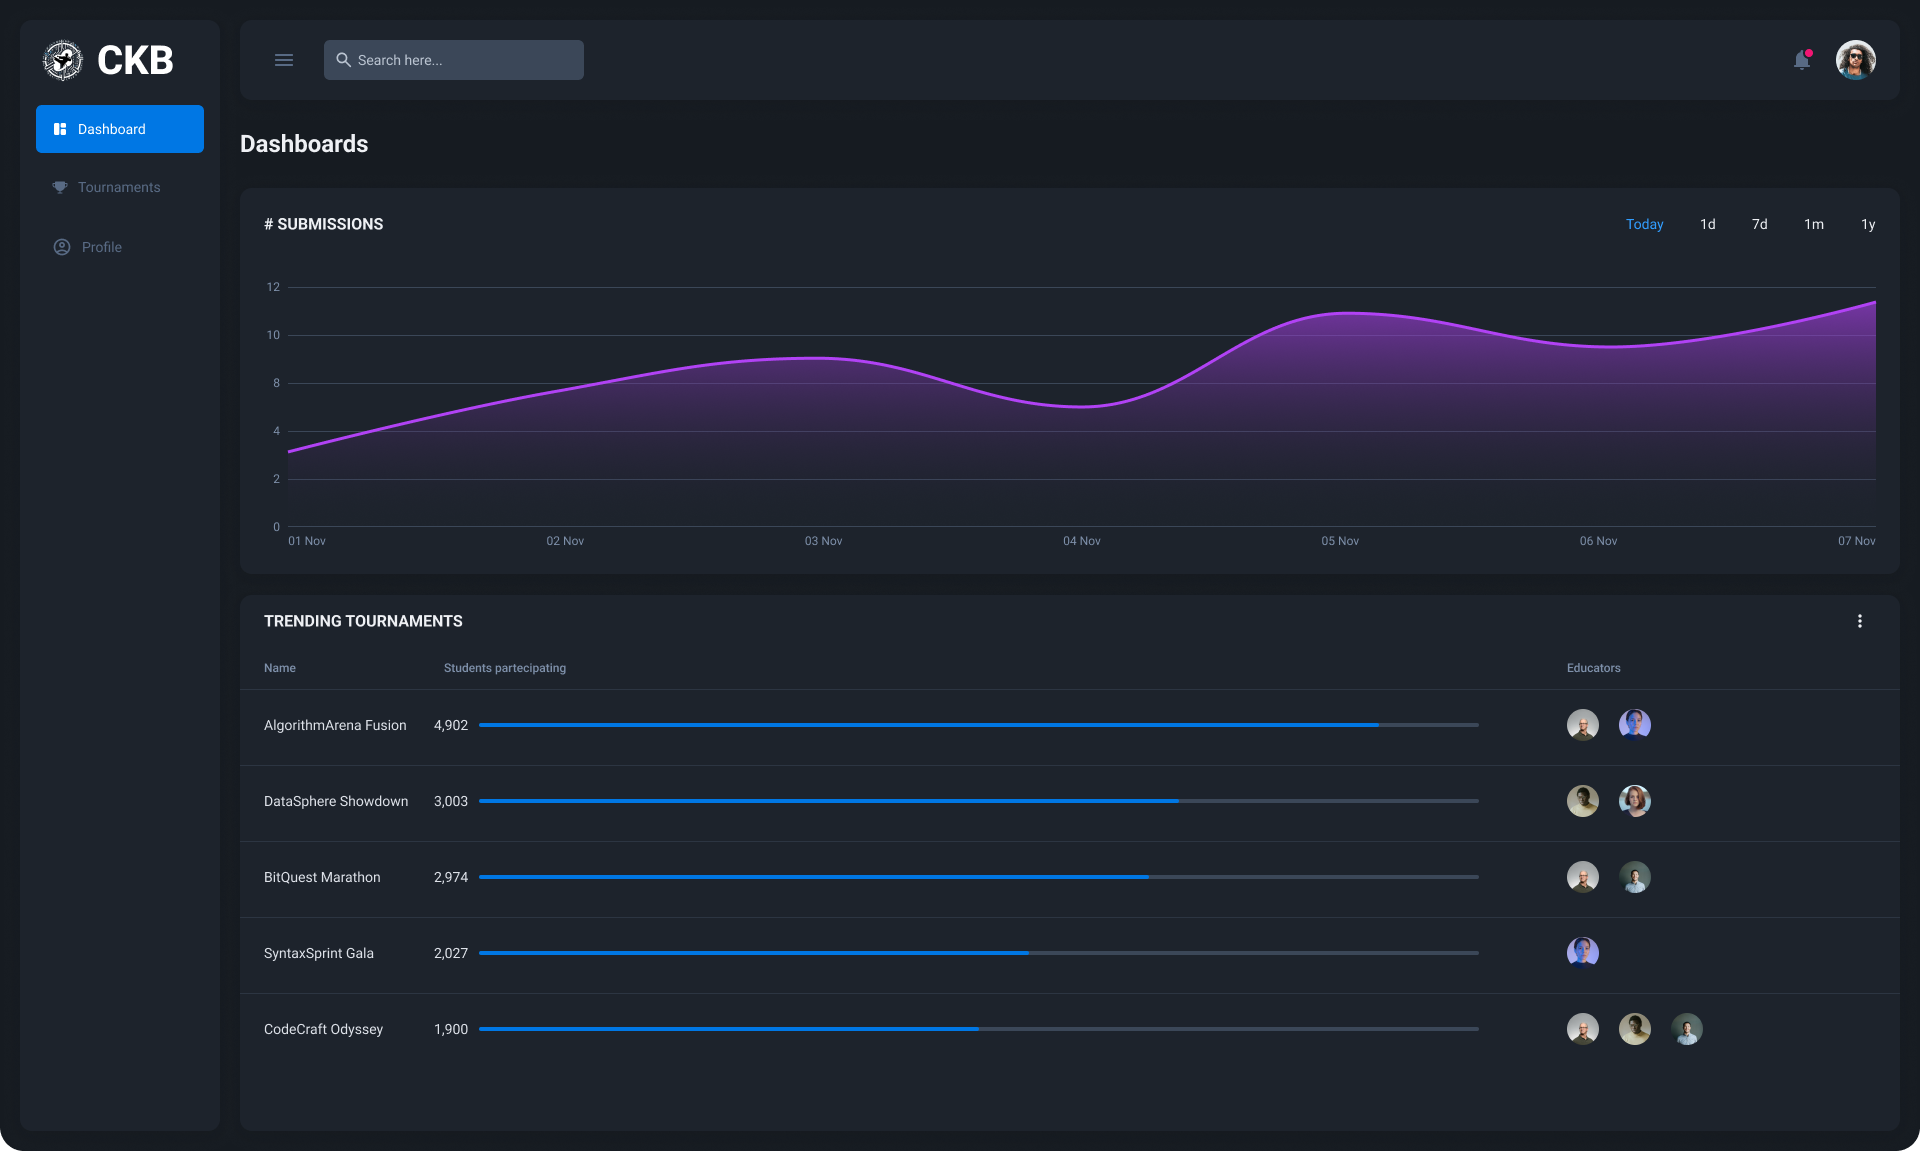
\includegraphics[width=\textwidth]{Images/Dashboard-Student.png}
    \caption{Student Dashboard}
    \label{fig:student-dashboard}
\end{figure}

\begin{figure}[H]
    \centering
    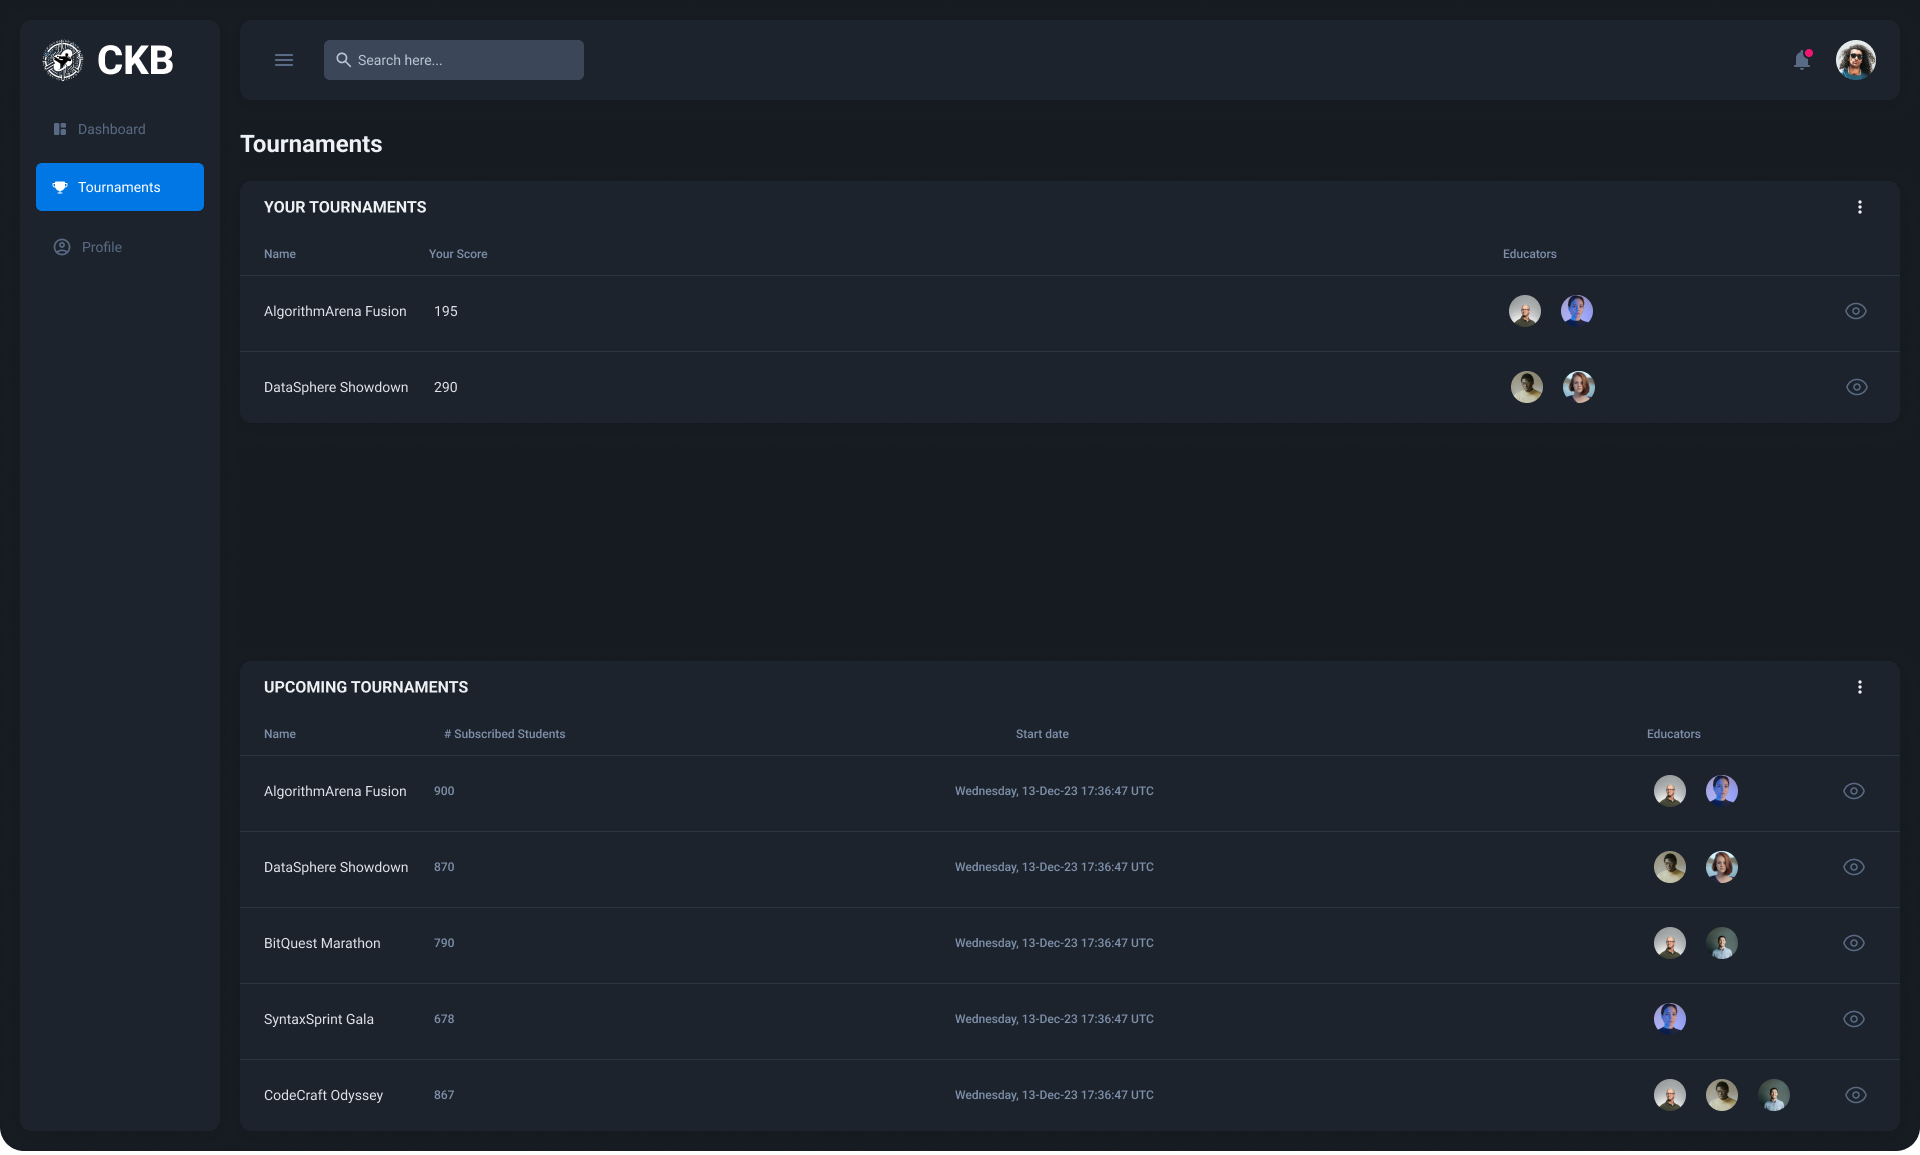
\includegraphics[width=\textwidth]{Images/Dashboard-Tournament.png}
    \caption{Student Dashboard Tournaments Tab}
    \label{fig:student-dashboard-tournaments}
\end{figure}

\begin{figure}[H]
    \centering
    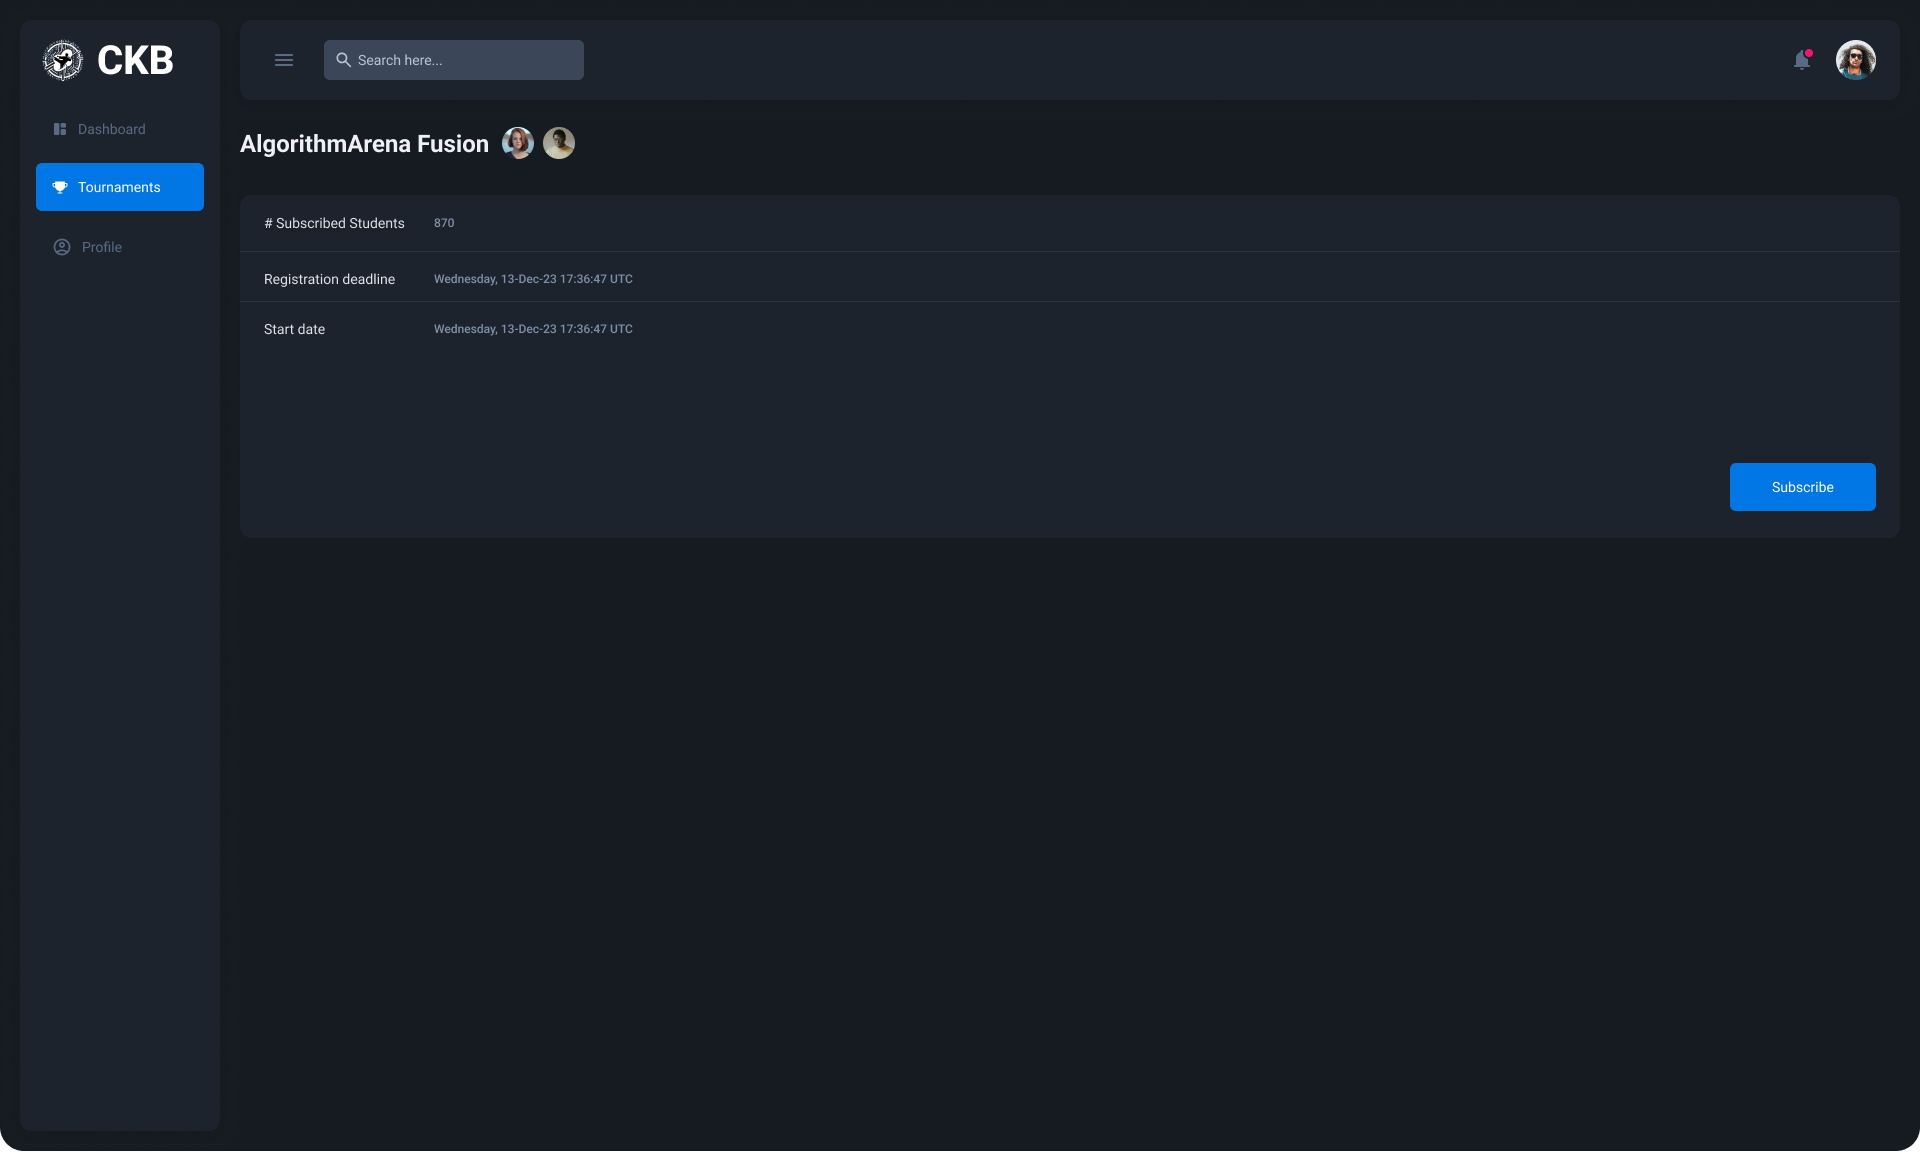
\includegraphics[width=\textwidth]{Images/Dashboard-Tournament-OverView.png}
    \caption{Student Dashboard Tournament OverView}
    \label{fig:student-Tournament-OverView}
\end{figure}

\begin{figure}[H]
    \centering
    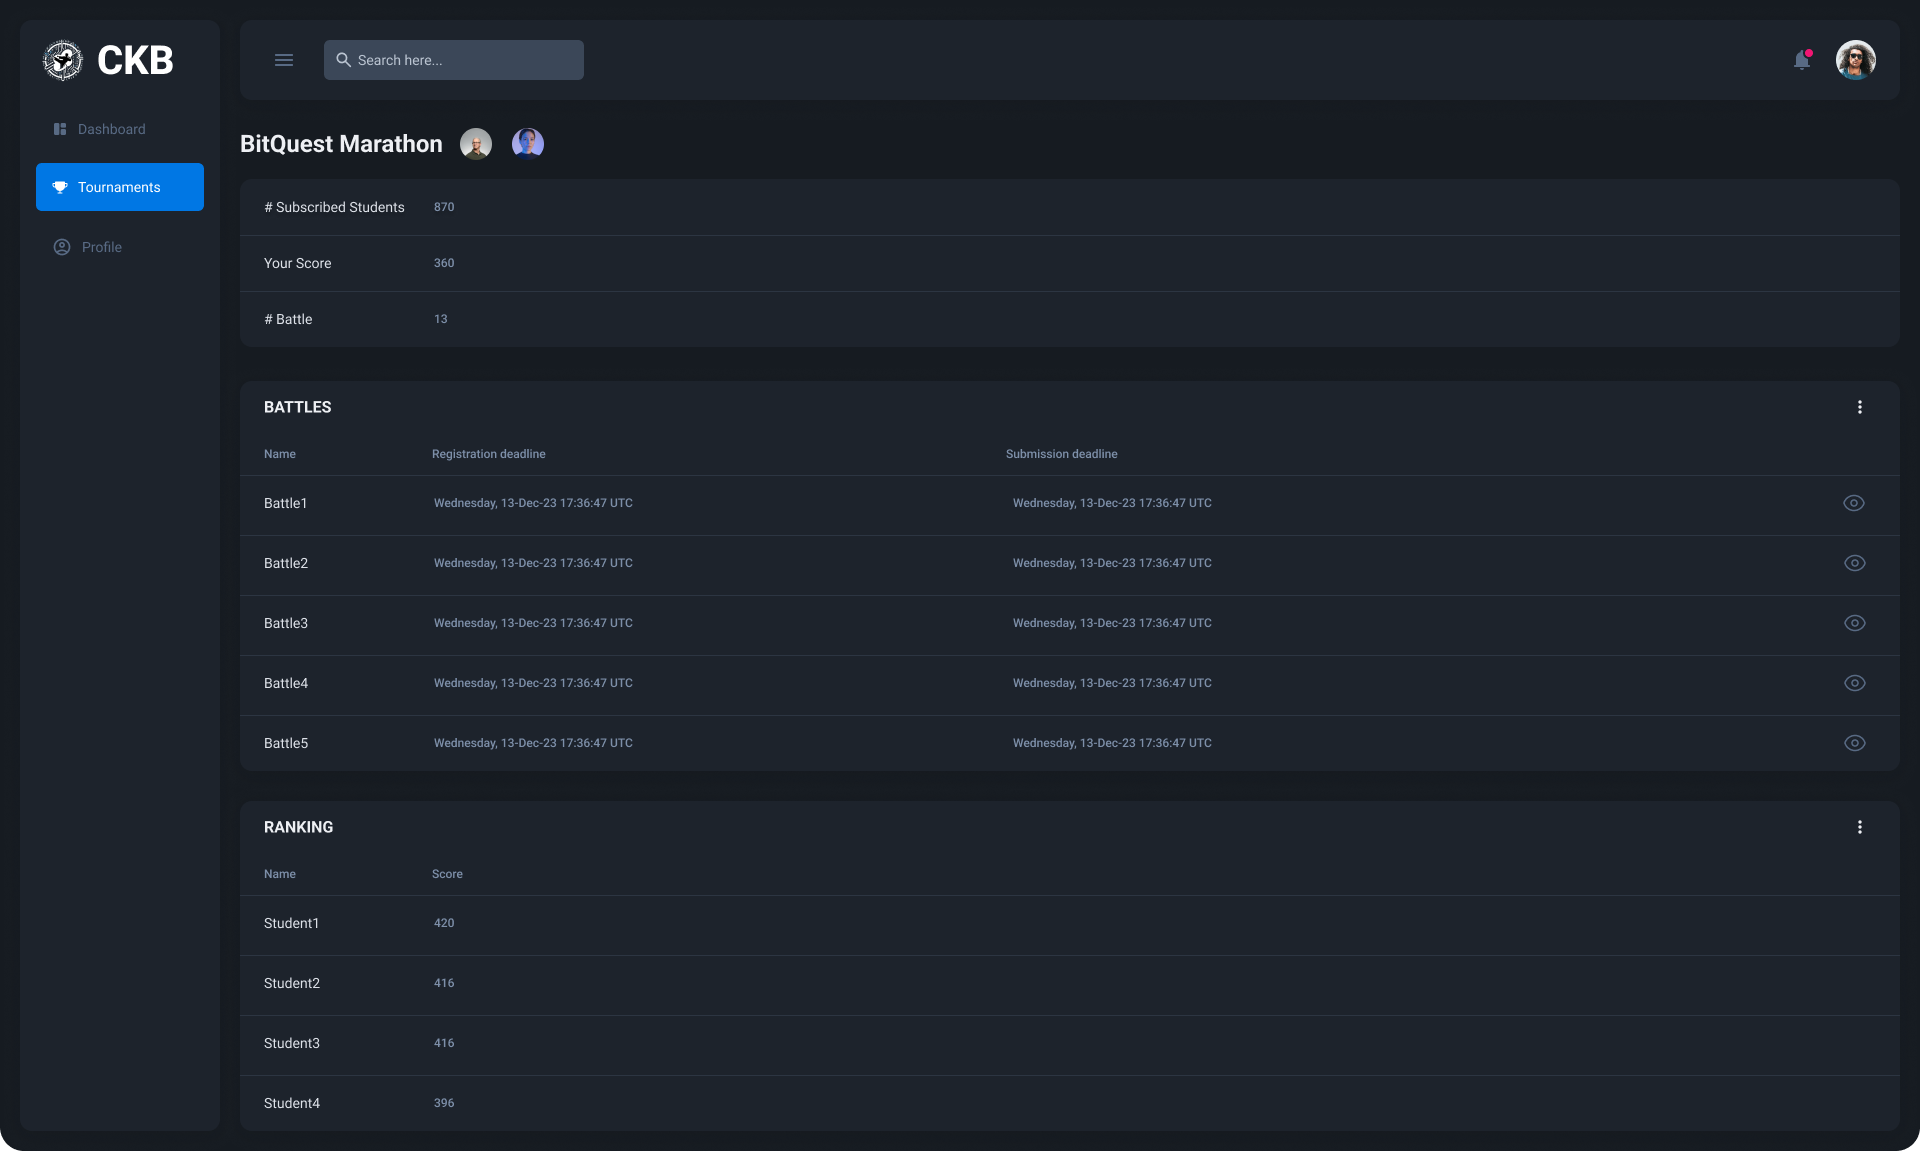
\includegraphics[width=\textwidth]{Images/Dashboard-Tournament-Ongoing.png}
    \caption{Student Dashboard Tournament Ongoing}
    \label{fig:student-Tournament-Ongoing}
\end{figure}

\begin{figure}[H]
    \centering
    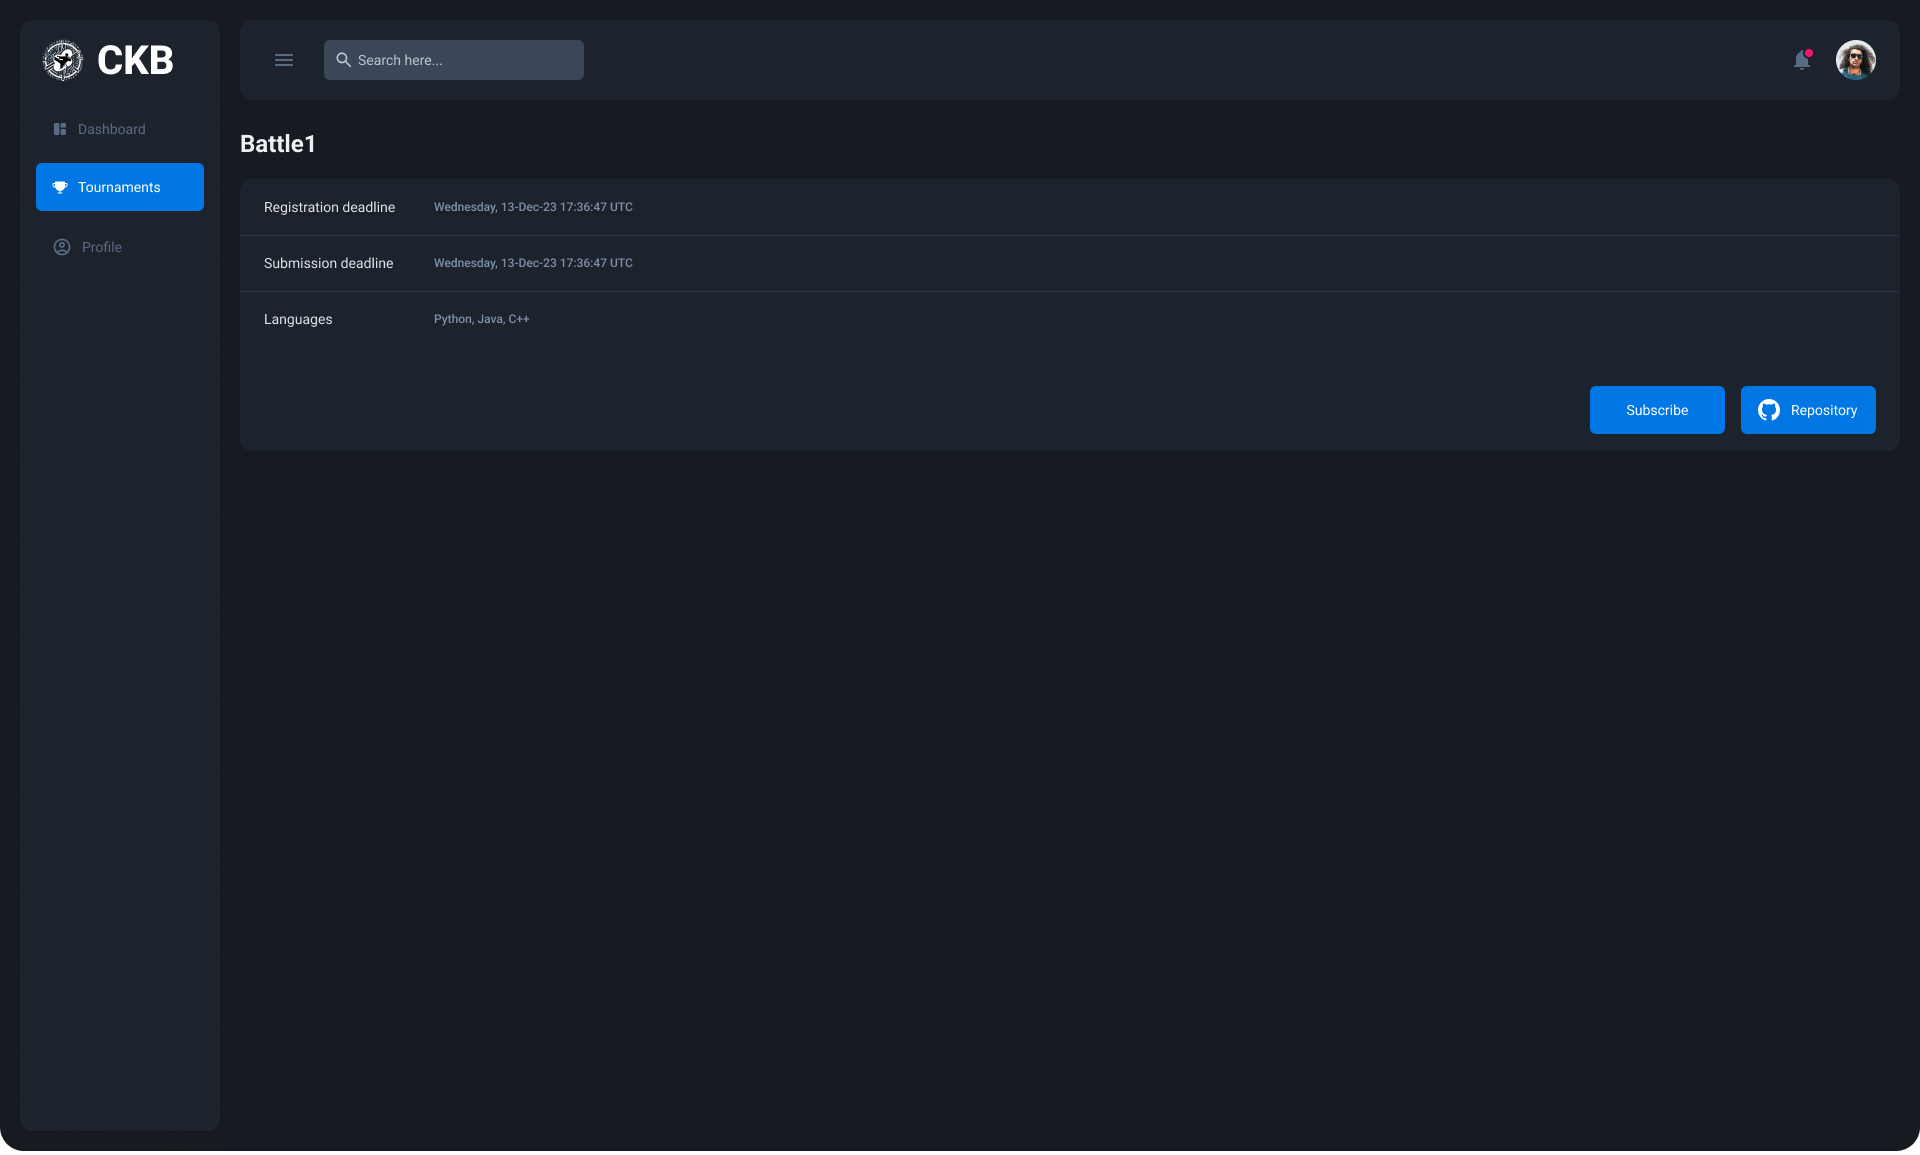
\includegraphics[width=\textwidth]{Images/Dashboard-Battle-Overview.png}
    \caption{Student Dashboard Battle Overview}
    \label{fig:student-Tournament-Completed}
\end{figure}


\subsubsection{Hardware Interfaces}
Since there is no particular hardware requirement for the system, the system will be able to run on any hardware that can run a web browser and has an internet connection.

\subsubsection{Software Interfaces}
The system in order to perform its functions does not require any interaction with other software systems.

\subsubsection{Communication Interfaces}
The system provides the functionality of automatic evaluation. This function requires the system to communicate with an external client that triggers this automatic actions. In particular, the system needs to expose an API that the GitHub Action set up by the students will call when a new commit is pushed.

\subsection{Functional Requirements}
This section specifies all the requirements that the system must satisfy in order to be considered complete and functional.

\begin{enumerate}[label=R\arabic*:]
    \item The system shall allow the user to register to the system
    \item The system shall allow the user to login to the system
    \item The system shall allow the educator to create a new tournament
    \item The system should allow the educator to create a new battle for a tournament
    \item The system shall allow the educator to set restrictions for a battle
    \item The system shall allow the educator to upload the code kata for a battle
    \item The system shall allow the student to subscribe to a tournament
    \item The system shall allow the student to subscribe to a battle
    \item The system shall create a repository for each battle such that is forkable by the students
    \item The system shall allow the student to create a team for a battle
    \item The system should allow the student to invite other students to join a team
    \item The system should notify students subscribed to the platform when a new tournament is created
    \item The system should notify students subscribed to a tournament when a new battle is created
    \item The system should notify students subscribed to a tournament when the system publishes the ranking of the tournament
    \item The system shall guarantee that the restrictions for a battle set by the educator are respected
    \item The system shall allow the educator that created a tournament to invite other educators to the tournament
    \item The system shall allow the educator to close a tournament
    \item The system should allow the educator to manually update the score of a team for a battle
    \item The system should allow GitHub to trigger the automatic evaluation of a submission
\end{enumerate}

\subsubsection{Use Cases Diagram}
\subsubsection*{Educator Use Diagram}
\begin{figure}[H]
    \centering
    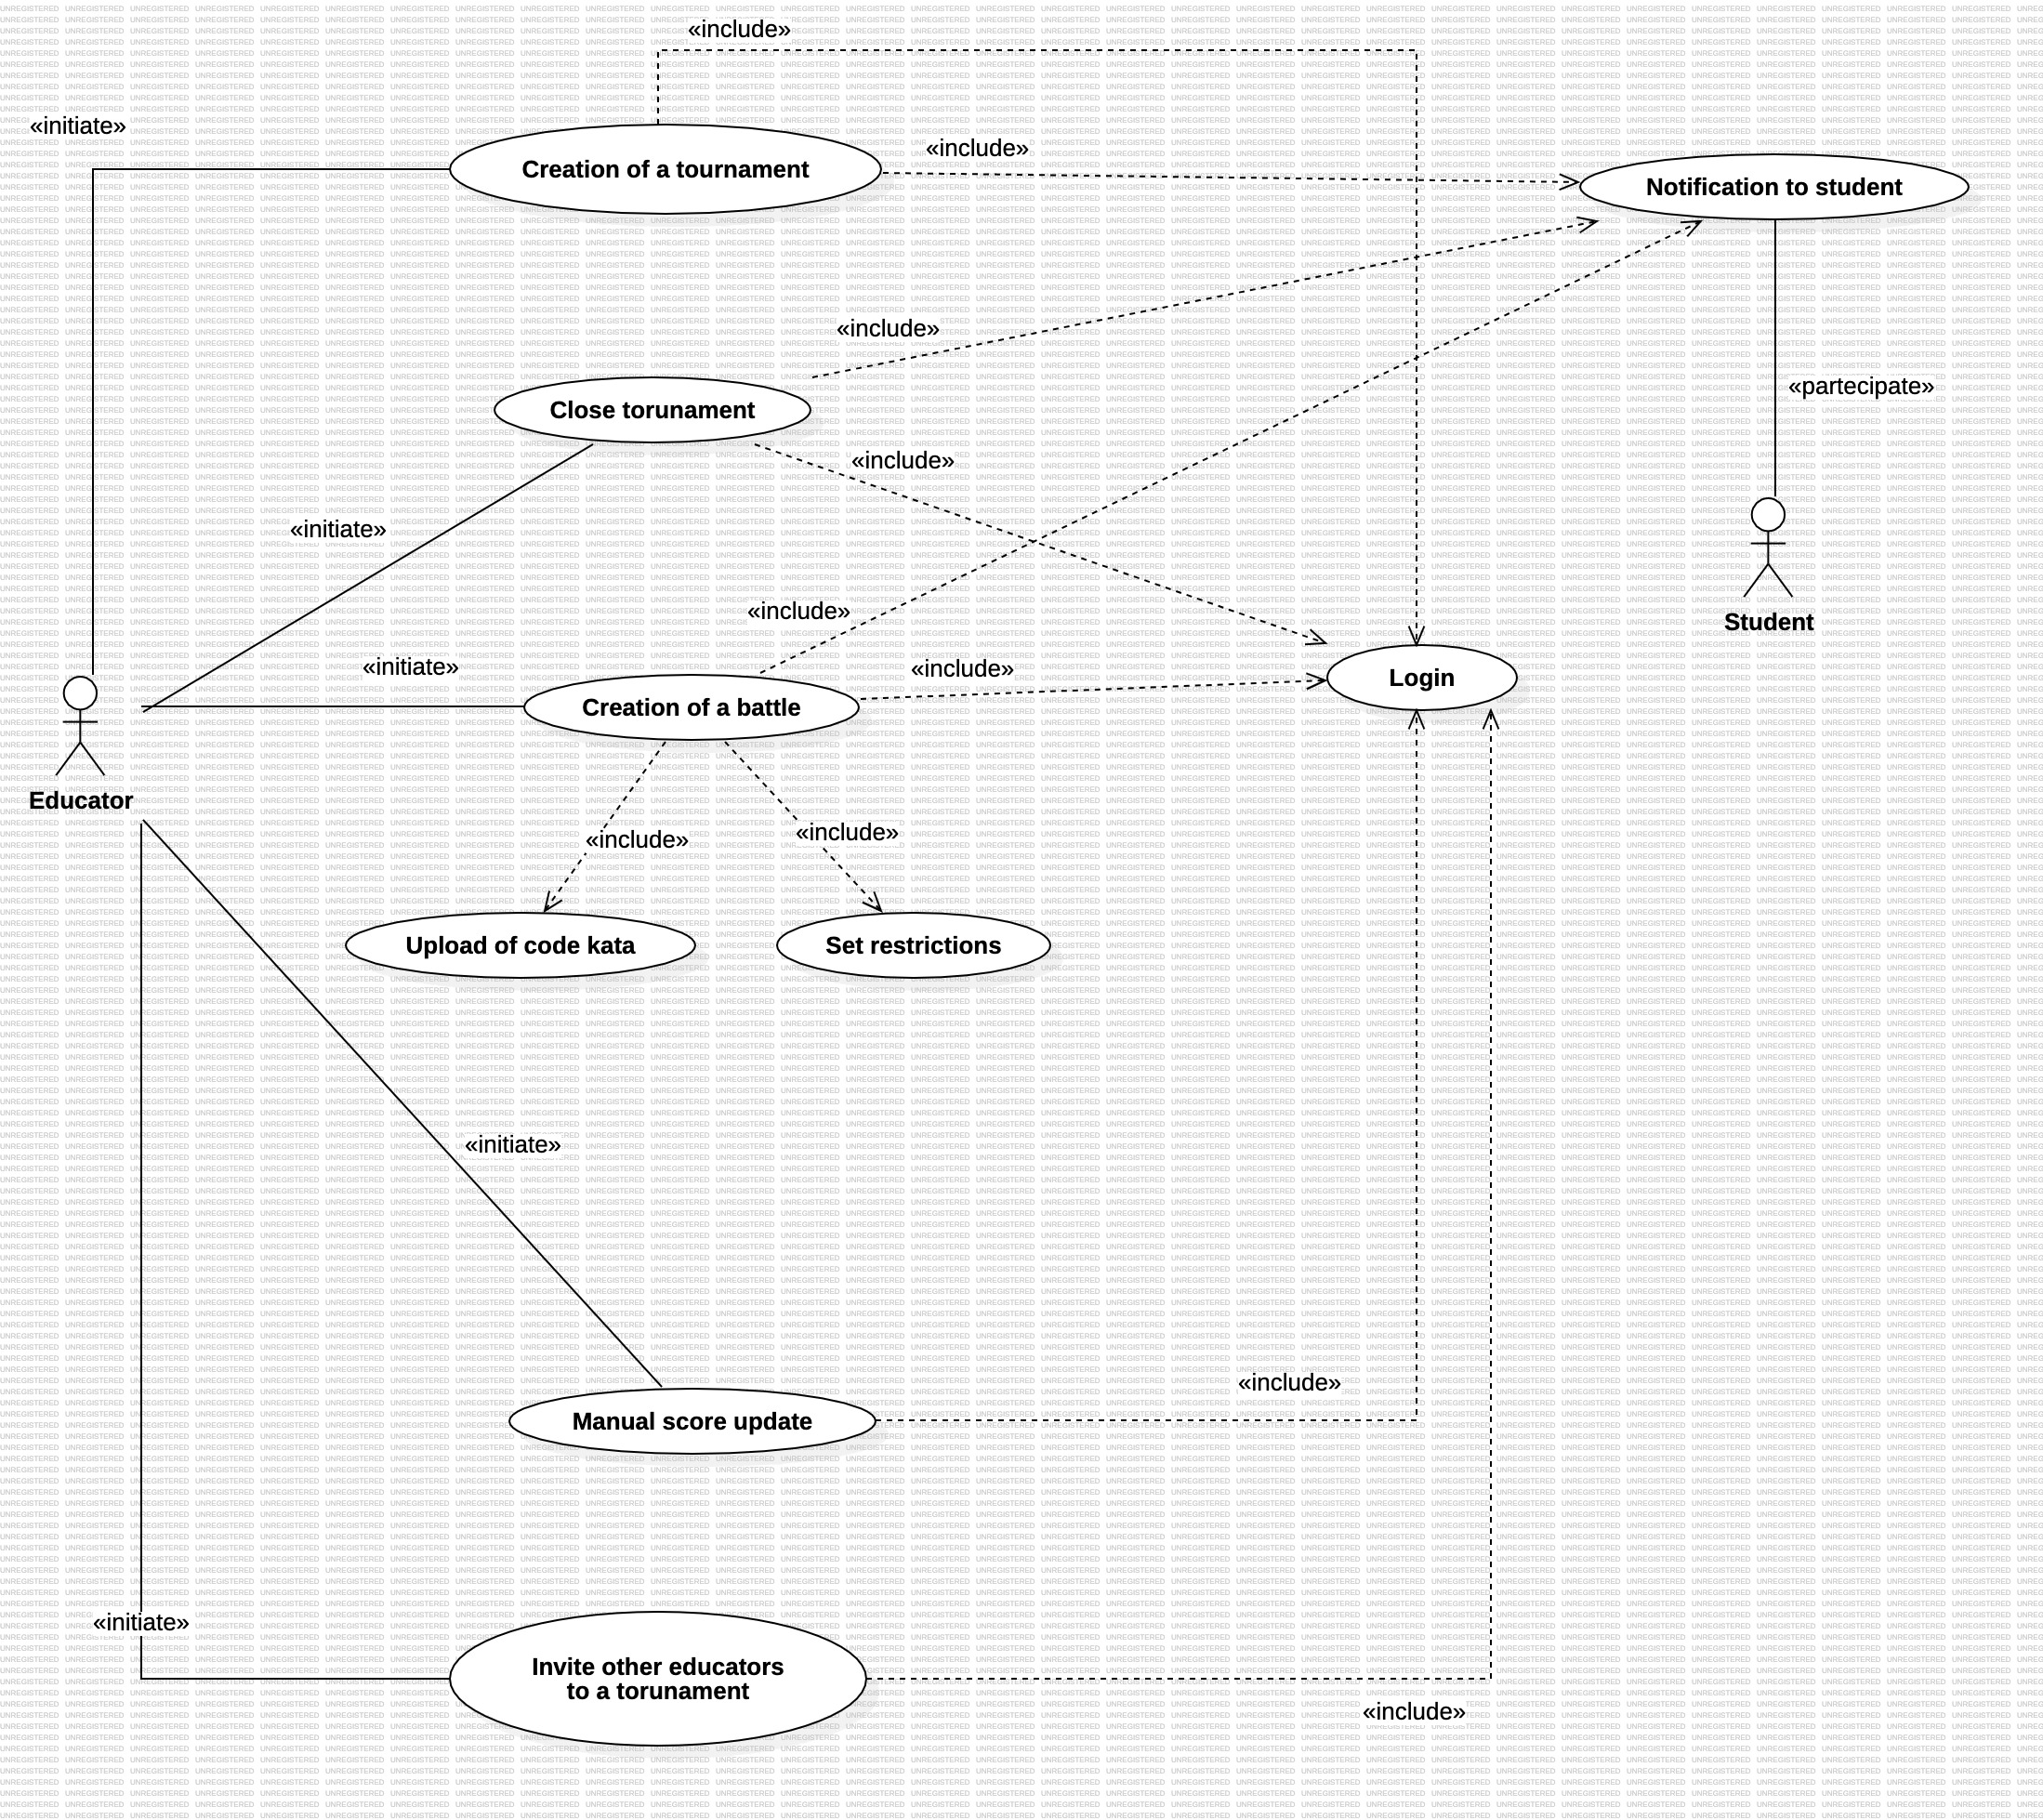
\includegraphics[width=\textwidth]{Diagrams/EducatorUseCaseDiagram.jpg}
    \caption{Educator Use Cases Diagram}
    \label{fig:student-use-diagram}
\end{figure}

\subsubsection*{Student Use Diagram}
\begin{figure}[H]
    \centering
    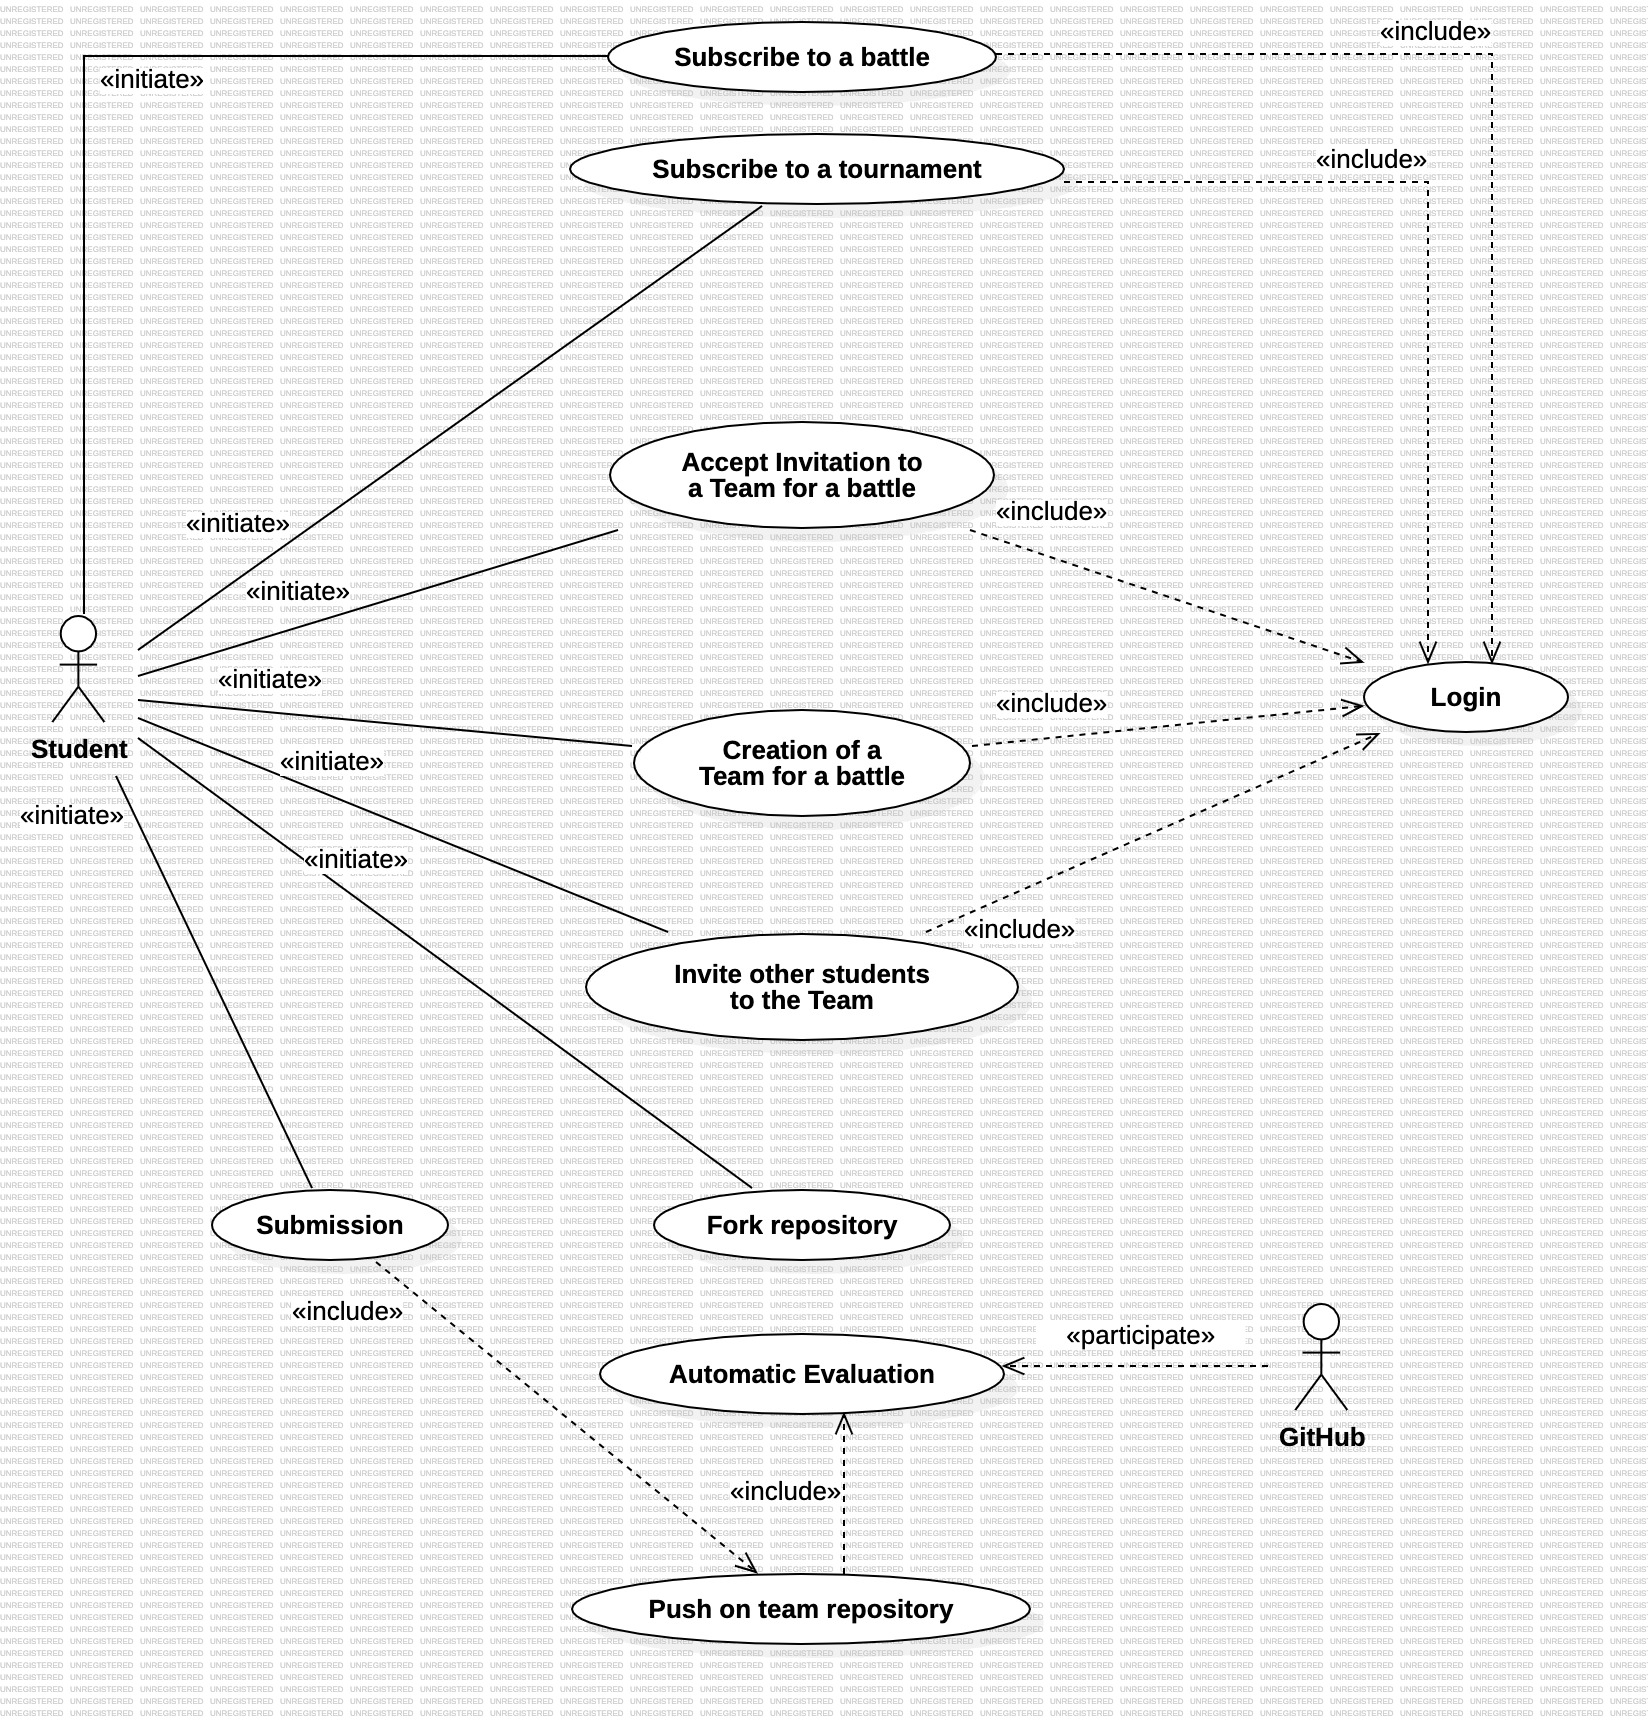
\includegraphics[width=\textwidth]{Diagrams/StudentUseCaseDiagram.jpg}
    \caption{Student Use Cases Diagram}
    \label{fig:student-use-diagram}
\end{figure}

\subsubsection{Use Cases}
\begin{enumerate}[label=UC\arabic*:]
    \item \textbf{User Login} \\
    \begin{tabular}{|p{3cm}|p{8cm}|}
        \hline
        Name & User Login \\
        \hline
        Actors & User \\
        \hline
        Entry condition & 
        \begin{itemize}
            \item The user is not logged in
            \item The user is registered to the system
            \item The user has a valid email and password
            \item The user has confirmed his email
        \end{itemize} 
        \\
        \hline
        Event flow &
        \begin{enumerate}[label=\arabic*.]
            \item The user enters his email and password
            \item The user clicks on the `Login' button
            \item The system checks the credentials
            \item The system logs in the user
            \item The user is redirected to the dashboard
        \end{enumerate}
        \\
        \hline
        Exit condition & 
        \begin{itemize}
            \item The user is logged in
        \end{itemize}
        \\
        \hline
        Exceptions &
        \begin{itemize}
            \item The user enters an invalid email or password
            \item The user has not confirmed his email
            \item The user is not registered to the system
        \end{itemize}
        \\
        \hline
    \end{tabular}
    \item \textbf{Creation of a tournament} \\
    \begin{tabular}{|p{3cm}|p{8cm}|}
        \hline
        Name & Creation of a tournament \\
        \hline
        Actors & Educator, Student \\
        \hline
        Entry condition &
        \begin{itemize}
            \item The Educator is subscribed to CKB platform
            \item The Student is subscribed to CKB platform
        \end{itemize}
        \\
        \hline
        Event flow & 
        \begin{enumerate}[label=\arabic*.]
            \item The Educator logs in to the system
            \item The Educator clicks on the `Create Tournament button
            \item The Educator fills the form with the information about the tournament, the registration deadline and the starting date
            \item The Educator clicks on the `Create button
            \item The system creates the tournament
            \item The system notifies the subscribed students about the creation of the new tournament
        \end{enumerate}
        \\
        \hline
        Exit condition & The Educator successfully created the torunament \\
        \hline
    \end{tabular}
    \item \textbf{Close a tournament} \\
    \begin{tabular}{|p{3cm}|p{8cm}|}
    \hline
    Name & Close a tournament \\
    \hline
    Actors & Educator, Student \\
    \hline
    Entry condition &
    \begin{itemize}
        \item The Educator is subscribed to CKB platform
        \item The Educator created a tournament
        \item The registration deadline of the tournament is passed
        \item The tournament is not closed
    \end{itemize}
    \\
    \hline
    Event flow &
    \begin{enumerate}[label=\arabic*.]
        \item The Educator logs in to the system
        \item The Educator goes to the tournament page in which he wants to close
        \item The Educator clicks on the `Close Tournament' button
        \item The system closes the tournament
        \item The system notifies the subscribed students about the closing of the tournament
    \end{enumerate}
    \\
    \hline
    Exit condition & The Educator successfully closed the tournament \\
    \hline
    Exceptions & The registration deadline of the tournament is not passed \\
    \hline
    \end{tabular}
    \item \textbf{Creation of a battle} \\
    \begin{tabular}{|p{3cm}|p{8cm}|}
        \hline
        Name & Creation of a battle \\
        \hline
        Actors & Educator, Student, GitHub \\
        \hline
        Entry condition &
        \begin{itemize}
            \item The Educator is subscribed to CKB platform
            \item The Student is subscribed to CKB platform
            \item The Educator created a tournament
            \item The Student is subscribed to the tournament
        \end{itemize}
        \\
        \hline
        Event flow & 
        \begin{enumerate}[label=\arabic*.]
            \item The Educator logs in to the system
            \item The Educator goes to the tournament page in which he wants to create a battle for
            \item The Educator clicks on the `Create Battle button
            \item The Educator fills the form with the registration deadline, submission deadline, minimum number of students per team, maximum number of students per team
            \item The Educator click the `Upload Code Kata' button and selects the files to upload
            \item The Educator clicks on the `Create button
            \item The system creates the battle
            \item GitHub creates a forkable repository for the battle
            \item The system sends the link of the repository to the subscribed students
            \item The system notifies the subscribed students about the creation of the new battle
        \end{enumerate}
        \\
        \hline
        Exit condition & The Educator successfully created the battle \\
        \hline
    \end{tabular}
    \item \textbf{Upload of code kata} \\
    \begin{tabular}{|p{3cm}|p{8cm}|}
        \hline
        Name & Upload of code kata \\
        \hline
        Actors & Educator \\
        \hline
        Entry condition &
        \begin{itemize}
            \item The Educator is subscribed to CKB platform
            \item The Educator is logged in
            \item The Educator created a tournament
            \item The Educator created a battle for the tournament
        \end{itemize}
        \\
        \hline
        Event flow &
        \begin{enumerate}[label=\arabic*.]
            \item The Educator goes to the tournament page in which he wants to upload the code kata
            \item The Educator selects the battle in which he wants to upload the code kata
            \item The Educator clicks on the `Upload Code Kata' button
            \item The Educator selects the files to upload
            \item The Educator clicks on the `Upload' button
            \item The system uploads the code kata
        \end{enumerate}
        \\
        \hline
        Exit condition & The code kata is uploaded \\
        \hline
        Exceptions & The Educator is not the creator of the tournament \\
        \hline
    \end{tabular}
    \item \textbf{Manual score update} \\
    \begin{tabular}{|p{3cm}|p{8cm}|}
        \hline
        Name & Manual score update \\
        \hline
        Actors & Educator \\
        \hline
        Entry condition &   
        \begin{itemize}
            \item The Educator is subscribed to CKB platform
            \item The Educator is logged in
            \item The Educator created a tournament
            \item The Educator created a battle for the tournament
        \end{itemize}
        \\
        \hline
        Event flow &
        \begin{enumerate}[label=\arabic*.]
            \item The Educator goes to the tournament page in which he wants to update the score
            \item The Educator selects the battle in which he wants to update the score
            \item The Educator clicks on the `Update Score' button
            \item The Educator selects the team for which he wants to update the score
            \item The Educator fills the form with the new score
            \item The Educator clicks on the `Update' button
        \end{enumerate}
        \\
        \hline
        Exit condition & The score is updated \\
        \hline
        Exceptions & The Educator is not the creator of the tournament \\
        \hline
    \end{tabular}
    \item \textbf{Invite other educators to a tournament} \\
    \begin{tabular}{|p{3cm}|p{8cm}|}
        \hline
        Name & Invite other educators to a tournament \\
        \hline
        Actors & Educator \\
        \hline
        Entry condition &
        \begin{itemize}
            \item The Educator is subscribed to CKB platform
            \item The Educator created a tournament
        \end{itemize}
        \\
        \hline
        Event flow & 
        \begin{enumerate}[label=\arabic*.]
            \item The Educator logs in to the system
            \item The Educator goes to the tournament page in which he wants to invite other educators
            \item The Educator clicks on the `Invite Educator' button
            \item The Educator fills the form with the email of the educator to invite
            \item The Educator clicks on the `Invite' button
            \item The system sends an email to the educator to invite
        \end{enumerate}
        \\
        \hline
        Exit condition &
        \begin{itemize}
            \item The Educator successfully invited the other educator to the tournament
            \item The invited educator can create battles for the tournament
        \end{itemize} \\
        \hline
        Exceptions & The invited educator is not subscribed to the platform \\
        \hline
    \end{tabular}
    \item \textbf{Notification to a student} \\
    \begin{tabular}{|p{3cm}|p{8cm}|}
        \hline
        Name & Notification to a student \\
        \hline
        Actors & Educator, Student \\
        \hline
        Entry condition &
        \begin{itemize}
            \item The Student is subscribed to CKB platform
        \end{itemize}
        \\
        \hline
        Event flow &
        \begin{enumerate}[label=\arabic*.]
            \item The Educator creates or closes a tournament or a battle
            \item The system notifies the subscribed students about the event
        \end{enumerate}
        \\
        \hline
        Exit condition & The student has received the notification   \\
        \hline
    \end{tabular}
    \item \textbf{Subscribe to a tournament} \\
    \begin{tabular}{|p{3cm}|p{8cm}|}
        \hline
        Name & Student subscribe to a tournament \\
        \hline
        Actors & Student \\
        \hline
        Entry condition &
        \begin{itemize}
            \item The Student is subscribed to CKB platform
            \item The Educator created a tournament
            \item The Student is not subscribed to the tournament
        \end{itemize}
        \\
        \hline
        Event flow &
        \begin{enumerate}[label=\arabic*.]
            \item The Student logs in to the system
            \item The Student goes to the tournament page in which he wants to subscribe
            \item The Student clicks on the `Subscribe' button
        \end{enumerate} \\
        \hline
        Exit condition & The student is subscibed to the tournament \\
        \hline
        Exceptions & The registration deadline of the tournament is passed so
        the student cannot subscribe to the tournament \\
        \hline
    \end{tabular}
    \item \textbf{Subscribe to a battle} \\
    \begin{tabular}{|p{3cm}|p{8cm}|}
        \hline
        Name & Student subscribe to a battle \\
        \hline
        Actors & Student \\
        \hline
        Entry condition &
        \begin{itemize}
            \item The Student is subscribed to CKB platform
            \item The Student is subscribed to the tournament in which the battle is
            \item The Student is not subscribed to the battle
        \end{itemize}
        \\
        \hline
        Event flow &
        \begin{enumerate}[label=\arabic*.]
            \item The Student logs in to the system
            \item The Student goes to the tournament page
            \item The Student selects the battle in which he wants to subscribe
            \item The Student clicks on the `Subscribe' button
        \end{enumerate} \\
        \hline
        Exit condition & The student is subscibed to the battle \\
        \hline
        Exceptions & The registration deadline of the battle is passed so the student cannot subscribe to the battle \\
        \hline
    \end{tabular}
    \item \textbf{Accept invitation to a team for a battle} \\
    \begin{tabular}{|p{3cm}|p{8cm}|}
        \hline
        Name & Accept invitation to a team for a battle \\
        \hline
        Actors & Student \\
        \hline
        Entry condition &
        \begin{itemize}
            \item The Student is subscribed to CKB platform
            \item The Student is subscribed to the tournament in which the battle is
            \item The Student is subscribed to the battle
            \item The Student is not in a team for the battle
        \end{itemize} \\
        \hline
        Event flow &
        \begin{enumerate}[label=\arabic*.]
            \item The Student logs in to the system
            \item The Student goes to the notification page
            \item The Student clicks on the `Accept Invitation' button
            \item The system adds the student to the team for the battle
        \end{enumerate} \\
        \hline
        Exit condition & The invited student is part of the team for the battle \\
        \hline
        Exceptions &
        \begin{itemize}
            \item The submission deadline of the battle is passed so the student cannot subscribe to the battle
            \item The maximum number of students per team is reached so the student cannot subscribe to the Battle
            \item The invitation is expired so the student cannot subscribe to the battle
        \end{itemize} \\
        \hline
    \end{tabular}
    \item \textbf{Creation of a team for a battle} \\
    \begin{tabular}{|p{3cm}|p{8cm}|}
        \hline
        Name & Creation of a team for a battle \\
        \hline
        Actors & Student \\
        \hline
        Entry condition &
        \begin{itemize}
            \item The Student is subscribed to CKB platform
            \item The Student is subscribed to the tournament in which the battle is
            \item The Student is subscribed to the battle
            \item The Student is not in a team for the battle
        \end{itemize} \\
        \hline
        Event flow &
        \begin{enumerate}[label=\arabic*.]
            \item The Student logs in to the system
            \item The Student goes to the tournament page
            \item The Student selects the battle in which he wants to create a team
            \item The Student clicks on the `Create Team' button
            \item The Student fills the form with the name of the team
            \item The Student clicks on the `Create' button
        \end{enumerate} \\
        \hline
        Exit condition & The student is part of the team for the battle \\
        \hline
        Exceptions & The submission deadline of the battle is passed so the student cannot subscribe to the battle \\
        \hline
    \end{tabular}
    \item \textbf{Invite other students to the team} \\
    \begin{tabular}{|p{3cm}|p{8cm}|}
        \hline
        Name & Invite other students to the team \\
        \hline
        Actors & Student \\
        \hline
        Entry condition &
        \begin{itemize}
            \item The Student is subscribed to CKB platform
            \item The Student is subscribed to the tournament in which the battle is
            \item The Student is subscribed to the battle
        \end{itemize} \\
        \hline
        Event flow &
        \begin{enumerate}[label=\arabic*.]
            \item The Student logs in to the system
            \item The Student goes to the tournament page
            \item The Student selects the battle in which he wants to invite other students
            \item The Student clicks on the `Invite people' button
            \item The Student fills the form with the email of the students to invite
            \item The Student clicks on the `Invite' button
        \end{enumerate} \\
        \hline
        Exit condition & The student has been successfully invited to the team \\
        \hline
        Exceptions & The student invited is not registered on the CKB platform so he will not receive the invitation \\
        \hline
    \end{tabular}
    \item \textbf{Fork repository of a battle} \\
    \begin{tabular}{|p{3cm}|p{8cm}|}
        \hline
        Name & Fork repository of a battle \\
        \hline
        Actors & Student \\
        \hline
        Entry condition &
        \begin{itemize}
            \item The Student is subscribed to CKB platform
            \item The Student is subscribed to the tournament in which the battle is
            \item The Student is subscribed to the battle
        \end{itemize} \\
        \hline
        Event flow &
        \begin{enumerate}[label=\arabic*.]
            \item The Student logs in to the system
            \item The Student goes to the tournament page
            \item The Student selects the battle in which he wants to fork the repository
            \item The Student clicks on the `Repository' button
            \item The system redirects the Student to the GitHub page of the repository to fork
        \end{enumerate} \\
        \hline
        Exit condition & The student has forked the repository \\
        \hline
        Exceptions & The submission deadline of the battle is passed so the student cannot fork the repository \\
        \hline
    \end{tabular}
    \item \textbf{Submission of a solution for a battle} \\
    \begin{tabular}{|p{3cm}|p{8cm}|}
        \hline
        Name & Submission of a solution for a battle \\
        \hline
        Actors & Student, GitHub \\
        \hline
        Entry condition &
        \begin{itemize}
            \item The Student is subscribed to CKB platform
            \item The Student is subscribed to the tournament in which the battle is
            \item The Student is subscribed to the battle
            \item The Student is part of a team for the battle
            \item The Student has forked the repository of the battle
            \item The Student set up the GitHub Action to trigger the automatic evaluation
        \end{itemize} \\
        \hline
        Event flow &
        \begin{enumerate}[label=\arabic*.]
            \item The Student writes the solution for the battle
            \item The Student pushes the solution on the team repository
            \item GitHub triggers the automatic evaluation
            \item The system evaluates the solution
            \item The system updates the score of the team
        \end{enumerate} \\
        \hline
        Exit condition & The team has got a new score for the battle \\
        \hline
        Exceptions & The submission deadline of the battle is passed so the student submission is not evaluated \\
        \hline
    \end{tabular}
    \item \textbf{Push on team repository} \\
    \begin{tabular}{|p{3cm}|p{8cm}|}
        \hline
        Name & Push on team repository \\
        \hline
        Actors & Student, GitHub \\
        \hline
        Entry condition &
        \begin{itemize}
            \item The Student is subscribed to CKB platform
            \item The Student is subscribed to the tournament in which the battle is
            \item The Student is subscribed to the battle
            \item The Student is part of a team for the battle
            \item The Student has forked the repository of the battle
        \end{itemize} \\
        \hline
        Event flow &
        \begin{enumerate}[label=\arabic*.]
            \item The Student writes the solution for the battle
            \item The Student pushes the solution on the team repository
            \item GitHub triggers the automatic evaluation
            \item The system evaluates the solution
            \item The system updates the score of the team
        \end{enumerate} \\
        \hline
        Exit condition & The team has got a new score for the battle \\
        \hline
        Exceptions &
        \begin{itemize}
            \item The submission deadline of the battle is passed so the student submission is not evaluated
            \item The Student has not set up the GitHub Action to trigger the automatic evaluation
        \end{itemize} \\
        \hline
    \end{tabular}
    \item \textbf{Automatic evaluation of a submission} \\
    \begin{tabular}{|p{3cm}|p{8cm}|}
        \hline
        Name & Automatic evaluation of a submission \\
        \hline
        Actors & GitHub \\
        \hline
        Entry condition &
        \begin{itemize}
            \item The Student is subscribed to CKB platform
            \item The Student is subscribed to the tournament in which the battle is
            \item The Student is subscribed to the battle
            \item The Student is part of a team for the battle
            \item The Student has forked the repository of the battle
            \item The Student set up the GitHub Action to trigger the automatic evaluation
            \item The Student has pushed the solution on the team repository
        \end{itemize} \\
        \hline
        Event flow &
        \begin{enumerate}[label=\arabic*.]
            \item GitHub triggers the automatic evaluation
            \item The system builds the project with the building tool associated with the battle
            \item The system runs the tests associated with the battle on the built project
            \item The system calculate the score of the submission
        \end{enumerate} \\
        \hline
        Exit condition & The team has got a new score for the battle \\
        \hline
        Exceptions & The submission deadline of the battle is passed so the student submission is not evaluated \\
        \hline
    \end{tabular}
\end{enumerate}

\subsubsection{Sequence diagrams}
\subsubsection*{[UC2] Creation of a tournament}
\begin{figure}[H]
    \centering
    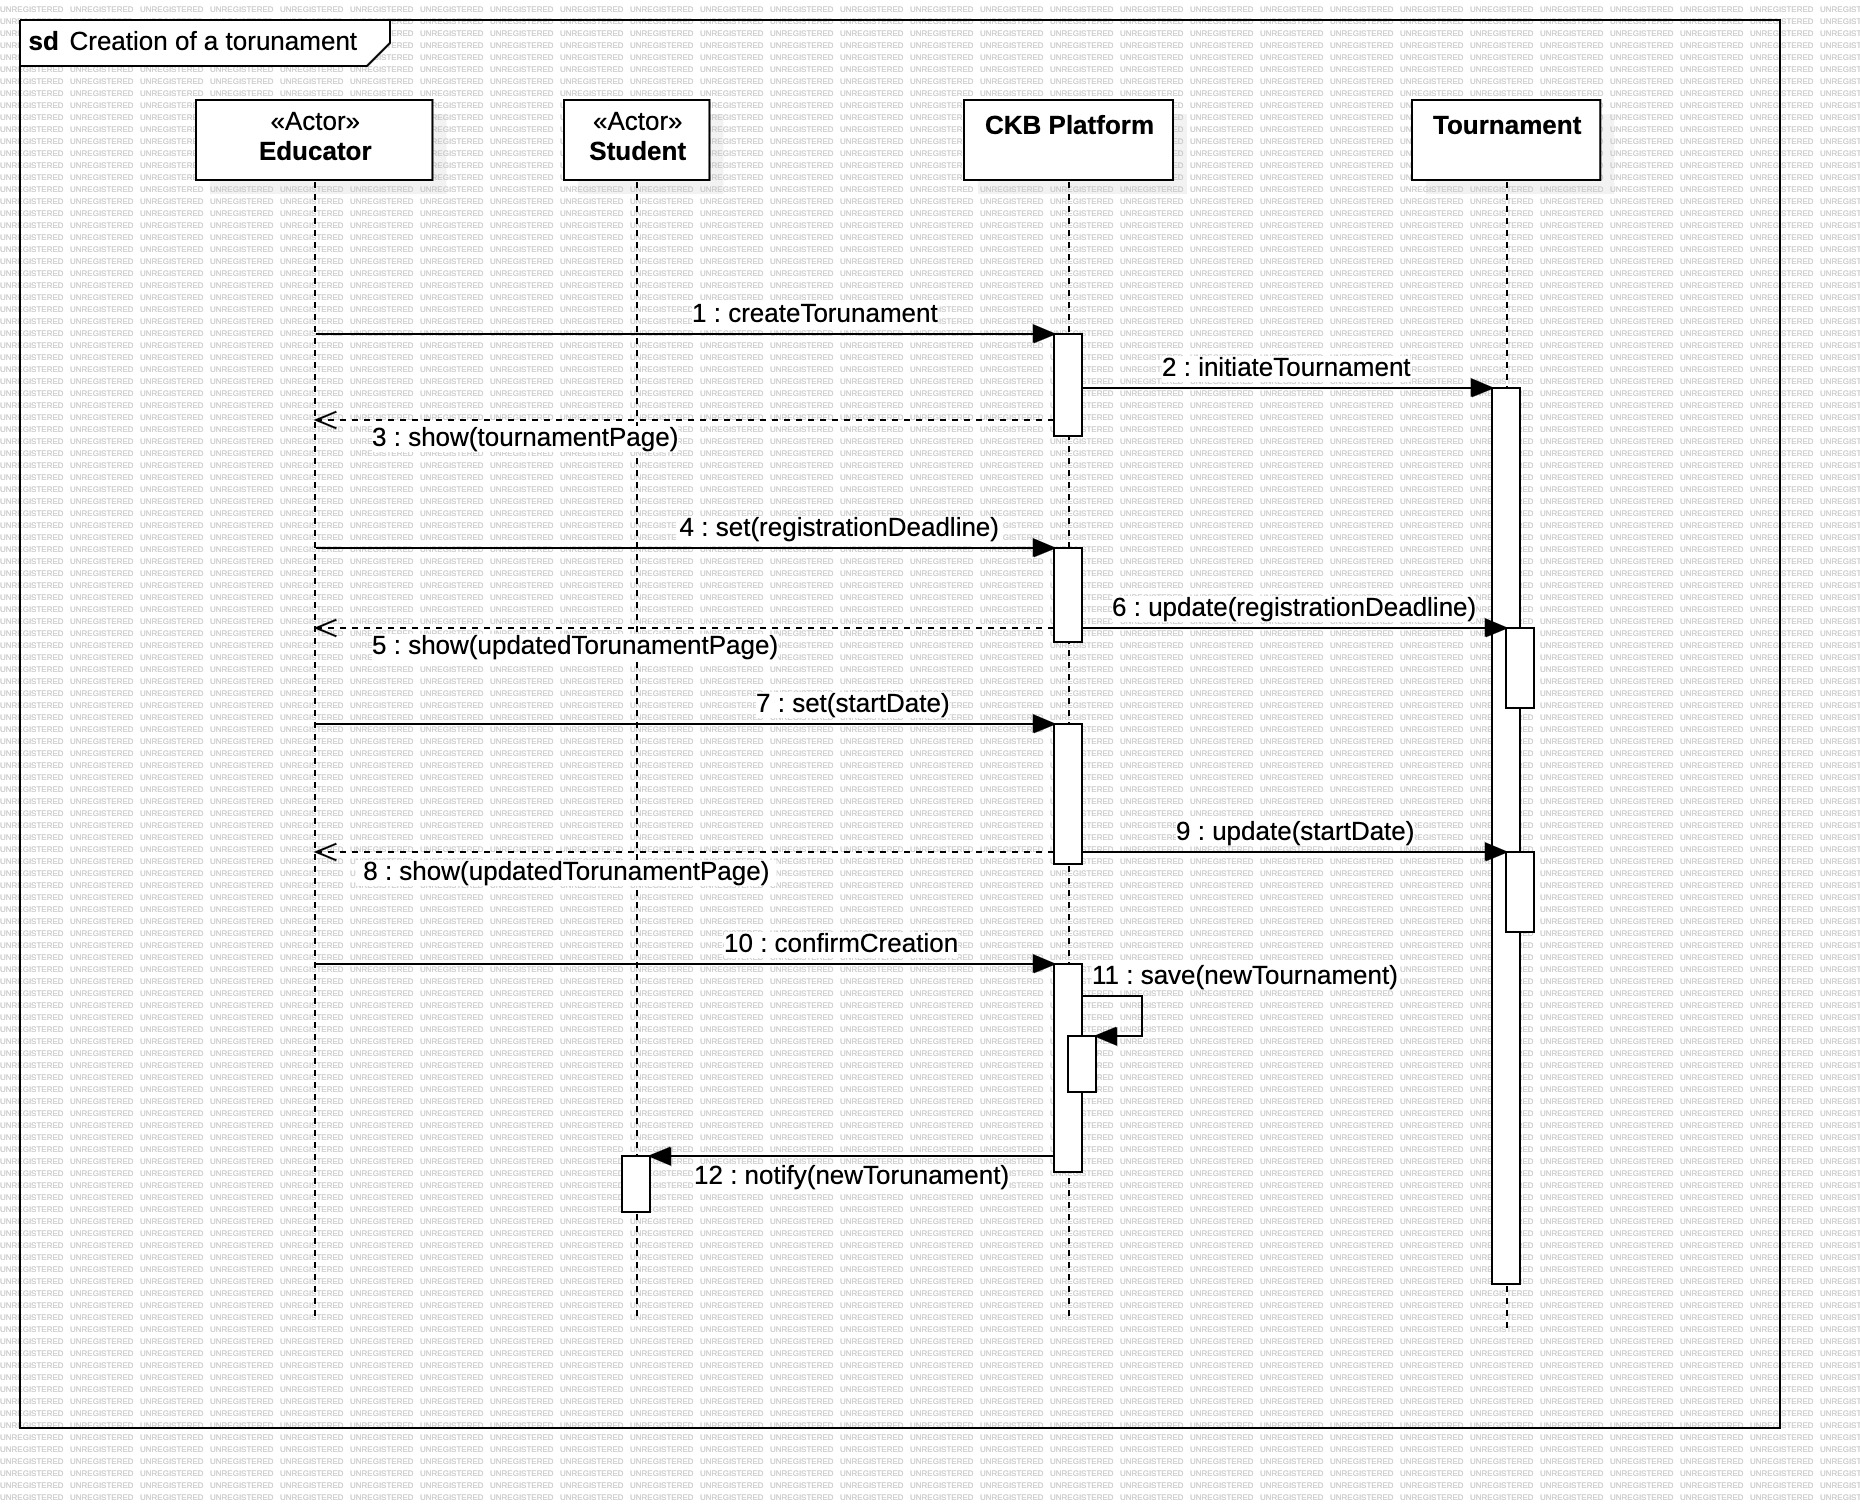
\includegraphics[width=\textwidth]{Diagrams/TournamentCreationSD.jpg}
    \caption{Sequence Diagram - Creation of a tournament}
    \label{fig:sequence-diagram-create-tournament}
\end{figure}

\subsubsection*{[UC4] Creation of a battle}
\begin{figure}[H]
    \centering
    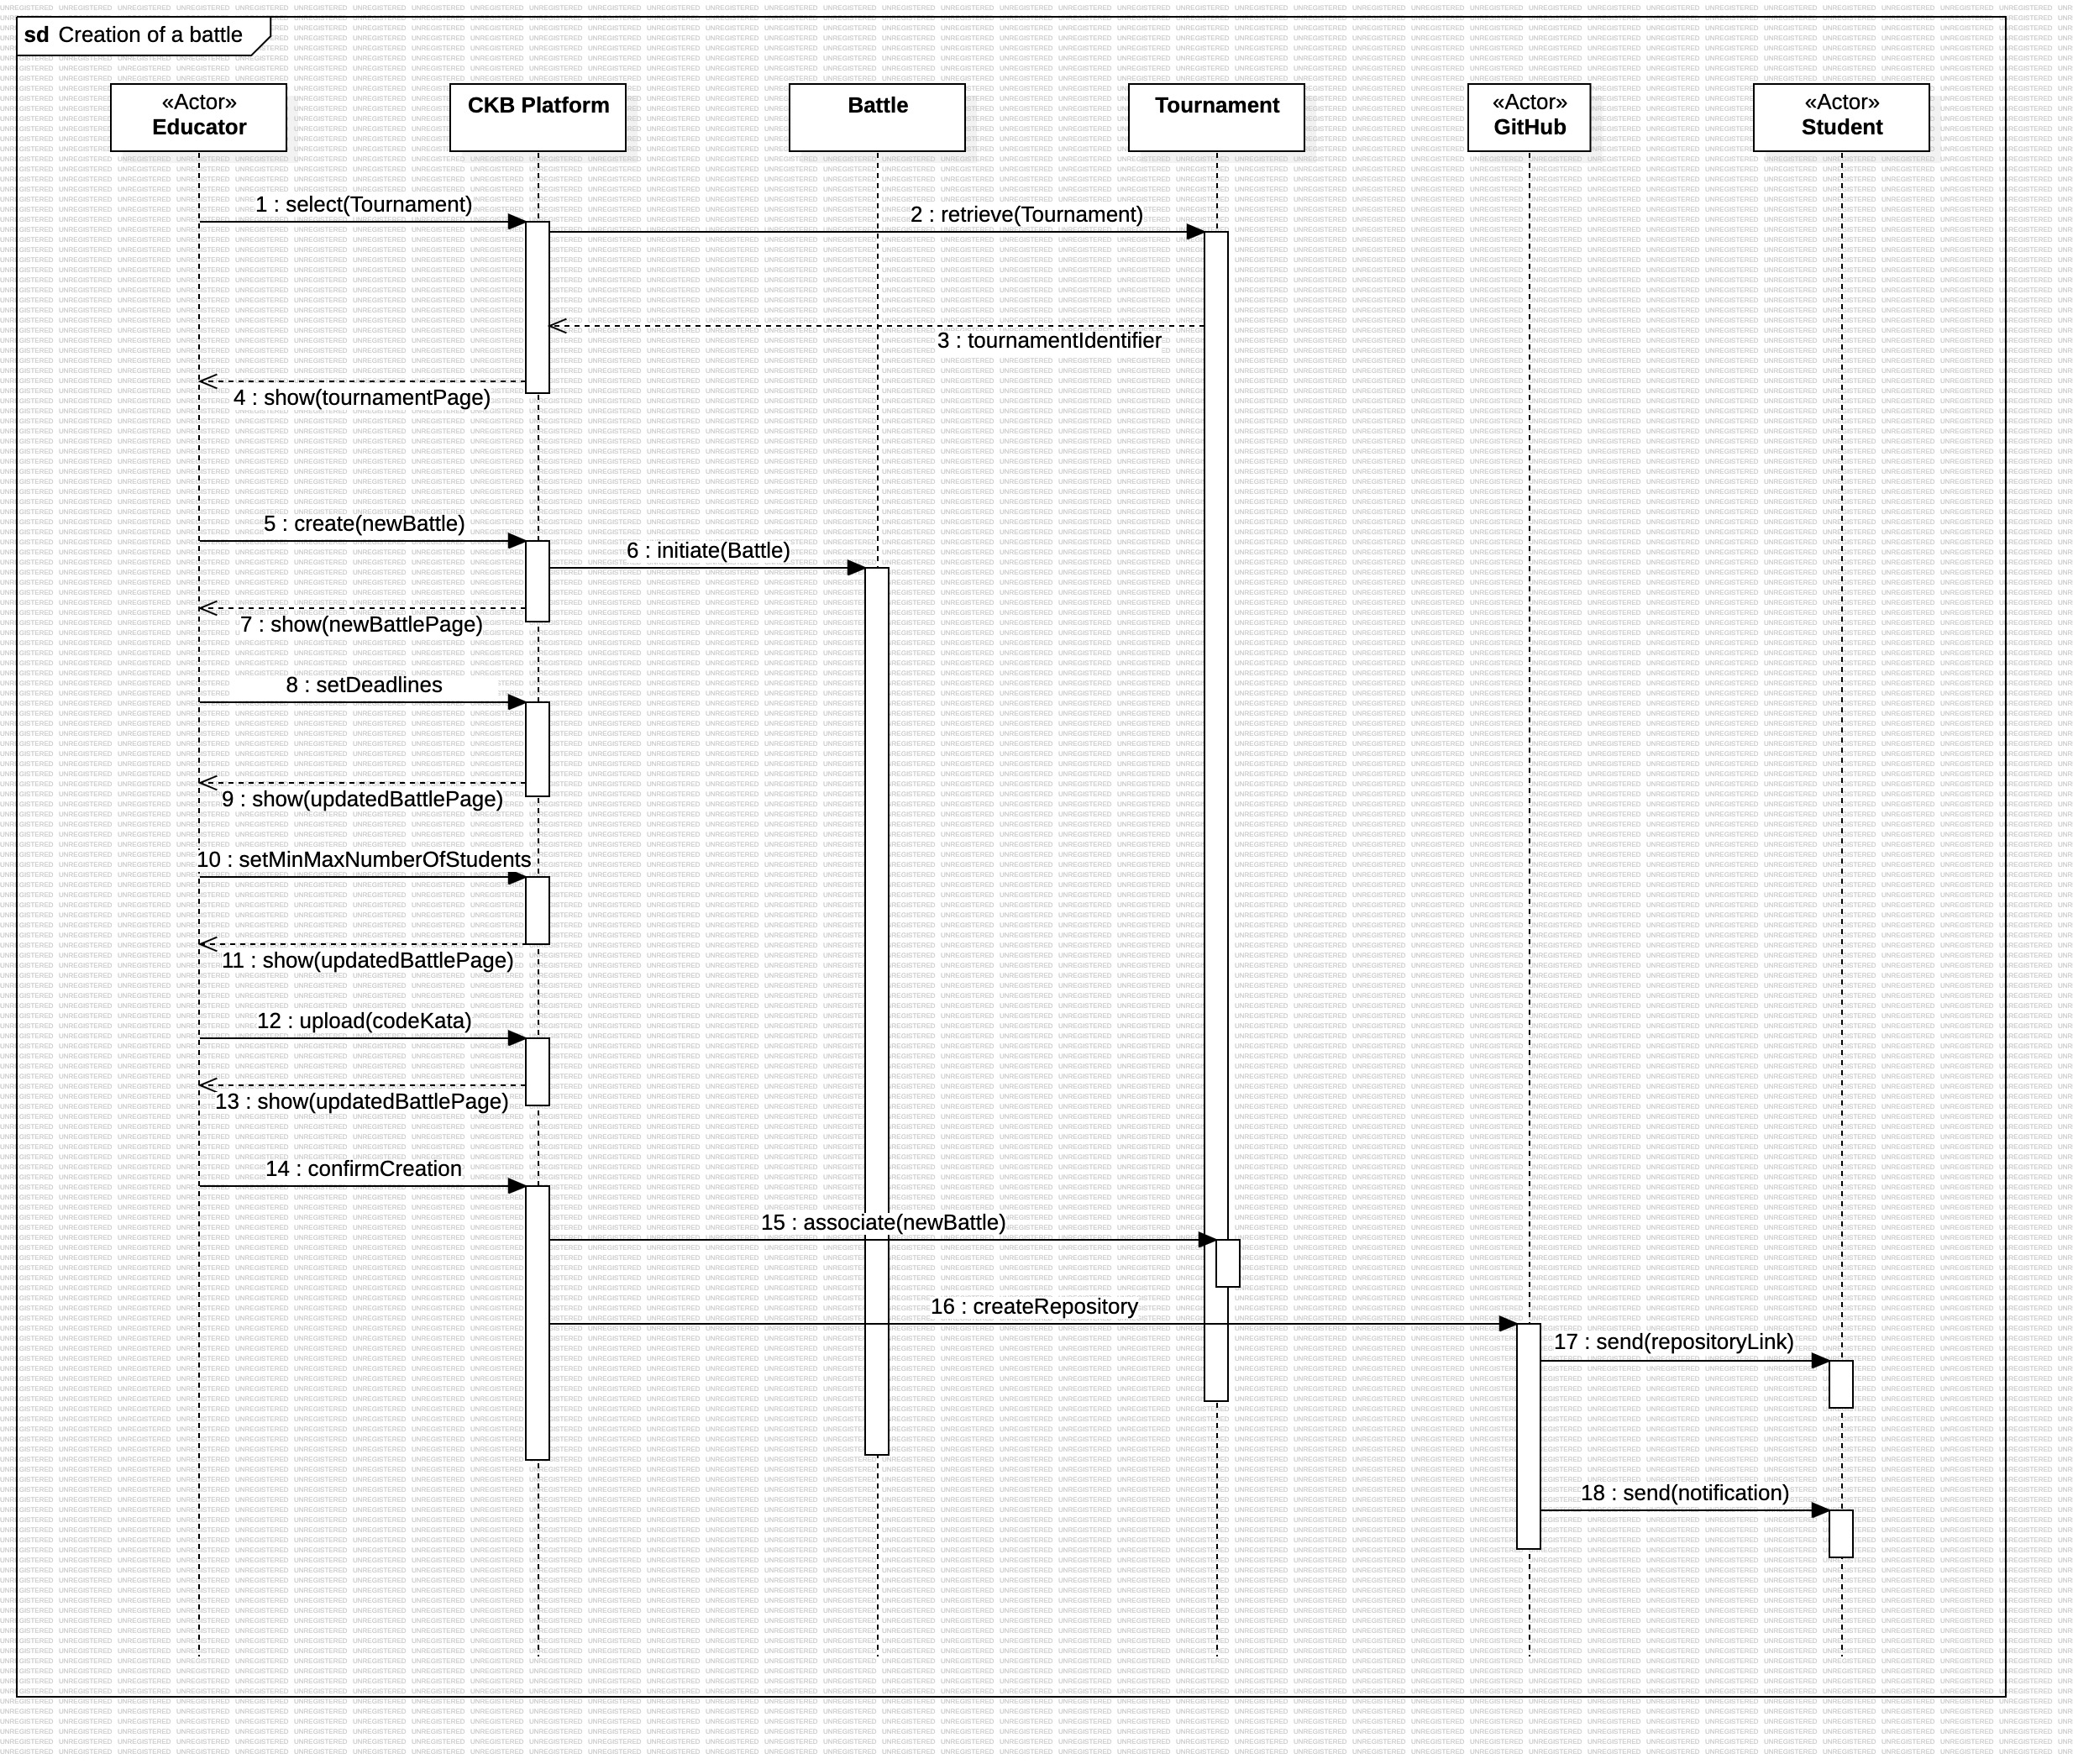
\includegraphics[width=\textwidth]{Diagrams/BattleCreation.jpg}
    \caption{Sequence Diagram - Creation of a battle}
    \label{fig:sequence-diagram-create-battle}
\end{figure}
\subsubsection*{[UC7] Invite othe educators to a tournament}
\begin{figure}[H]
    \centering
    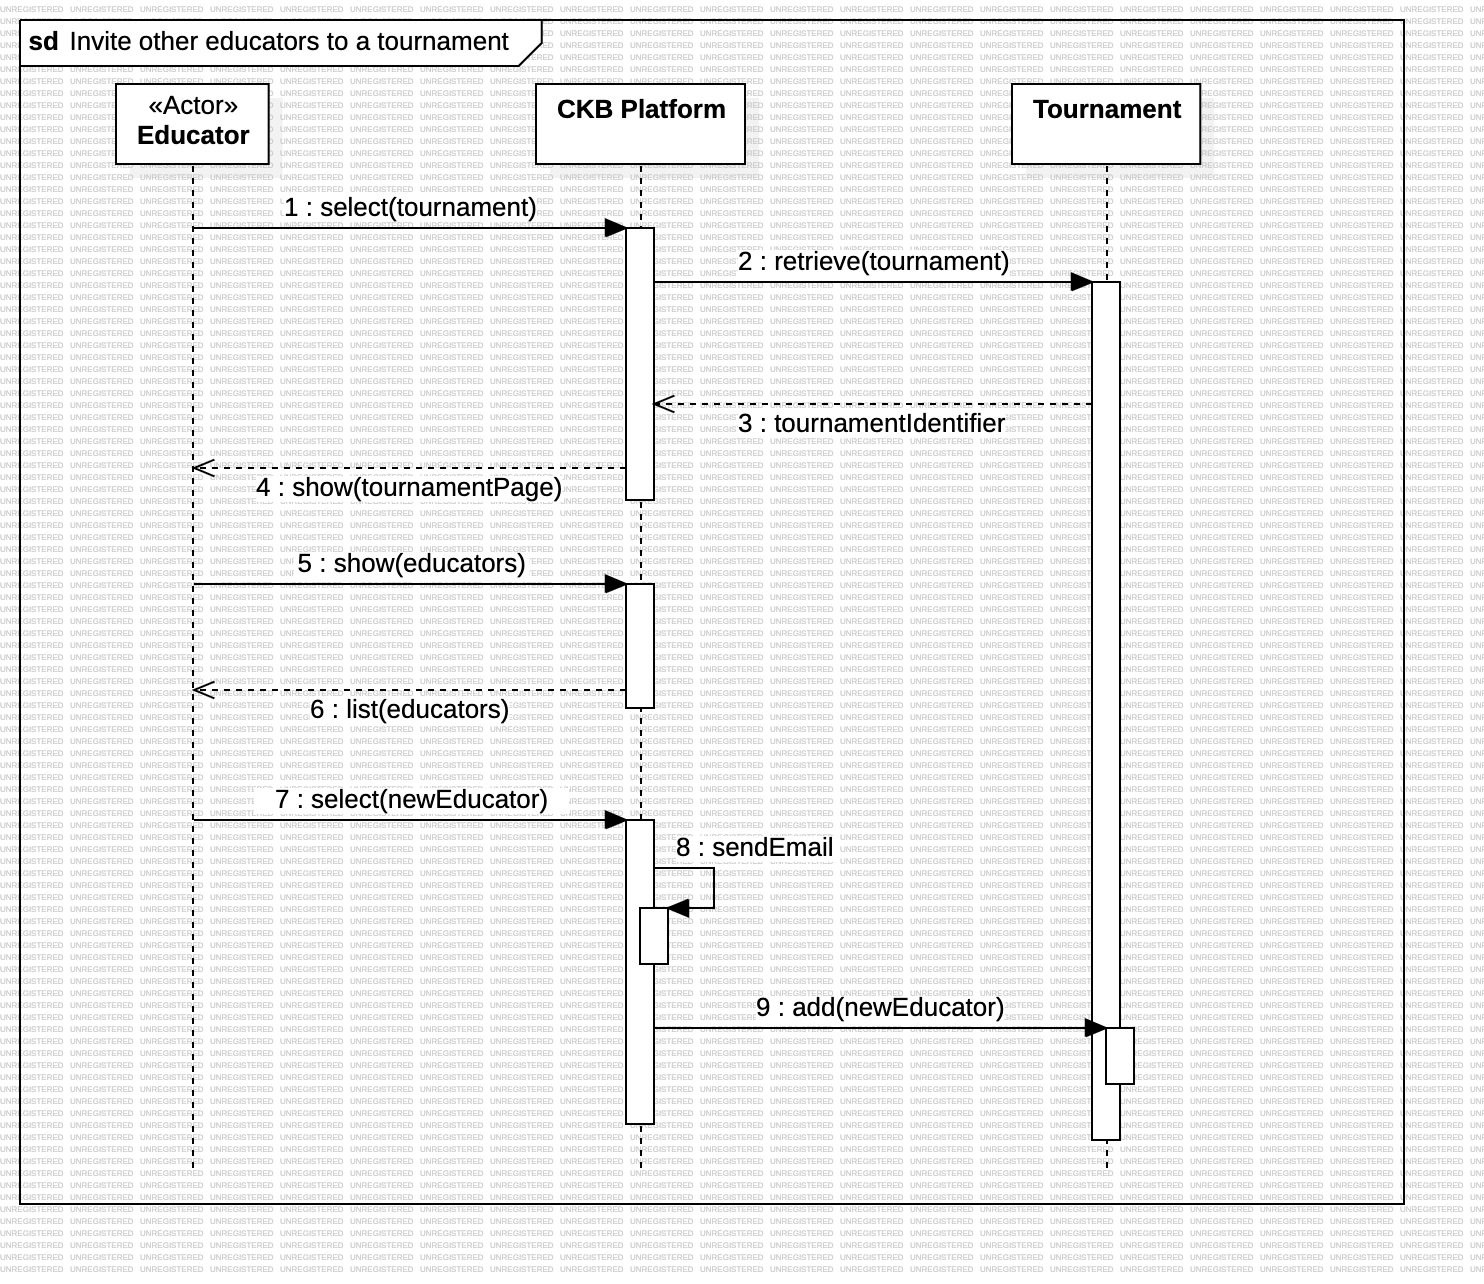
\includegraphics[width=\textwidth]{Diagrams/InviteEducators.jpg}
    \caption{Sequence Diagram - Invite other educators to a tournament}
    \label{fig:sequence-diagram-invite-educator}
\end{figure}
\subsubsection*{[UC9] Subscribe to a tournament}
\begin{figure}[H]
    \centering
    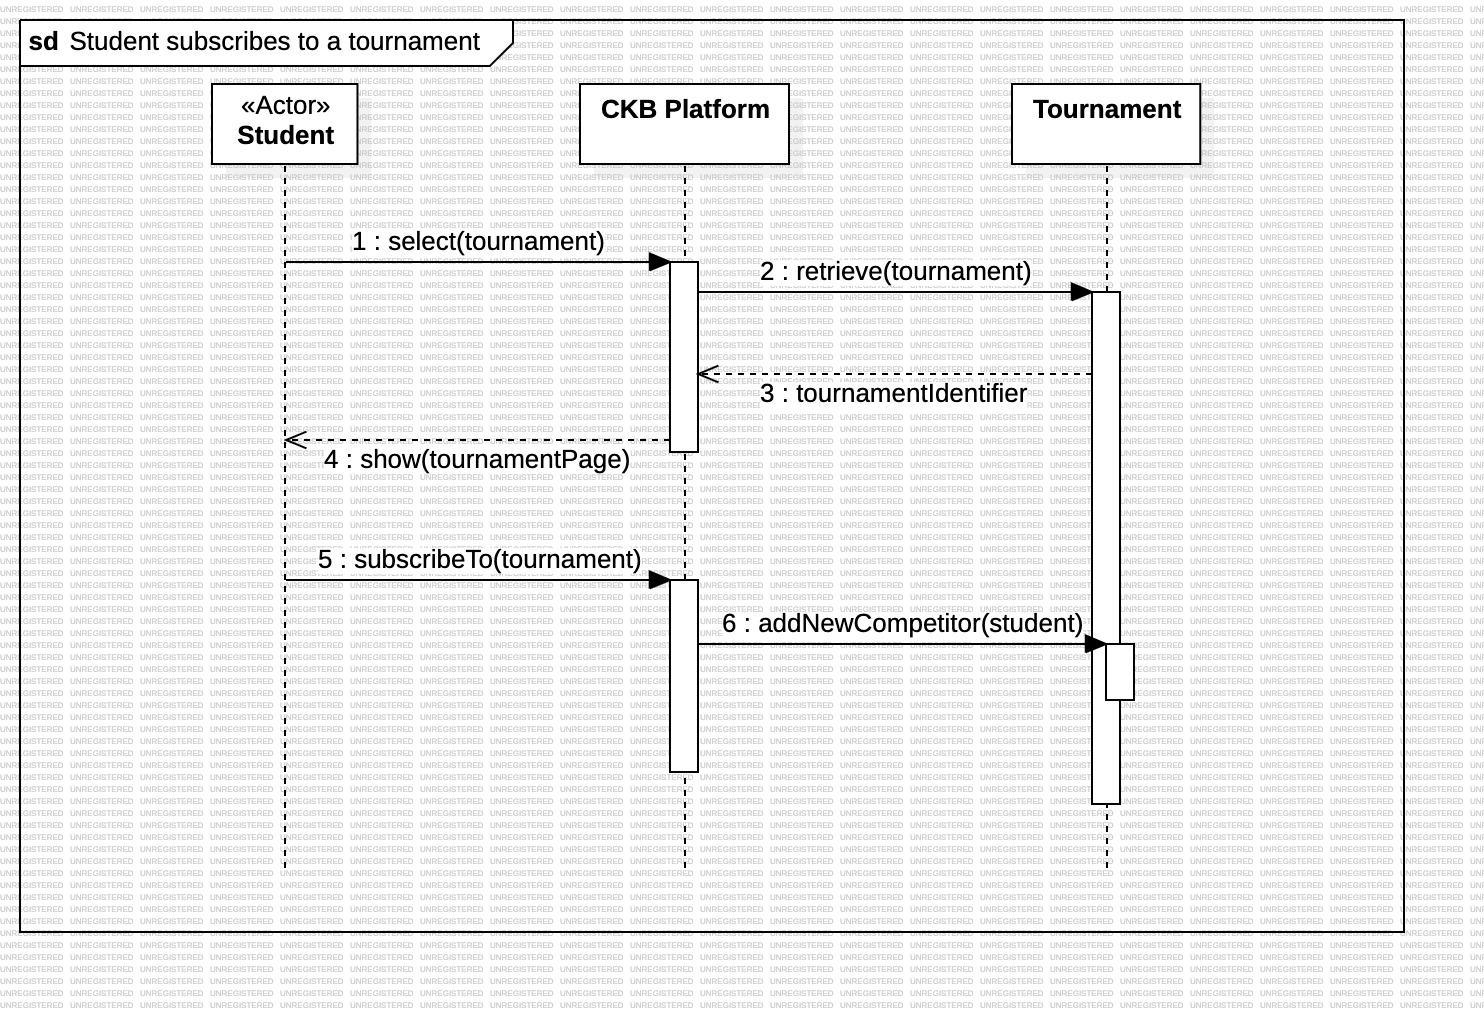
\includegraphics[width=\textwidth]{Diagrams/StudentSubscription.jpg}
    \caption{Sequence Diagram - Subscribe to a tournament}
    \label{fig:sequence-diagram-subscribe-tournament}
\end{figure}
\subsubsection*{[UC11] Accept invitation to a team for a battle}
\begin{figure}[H]
    \centering
    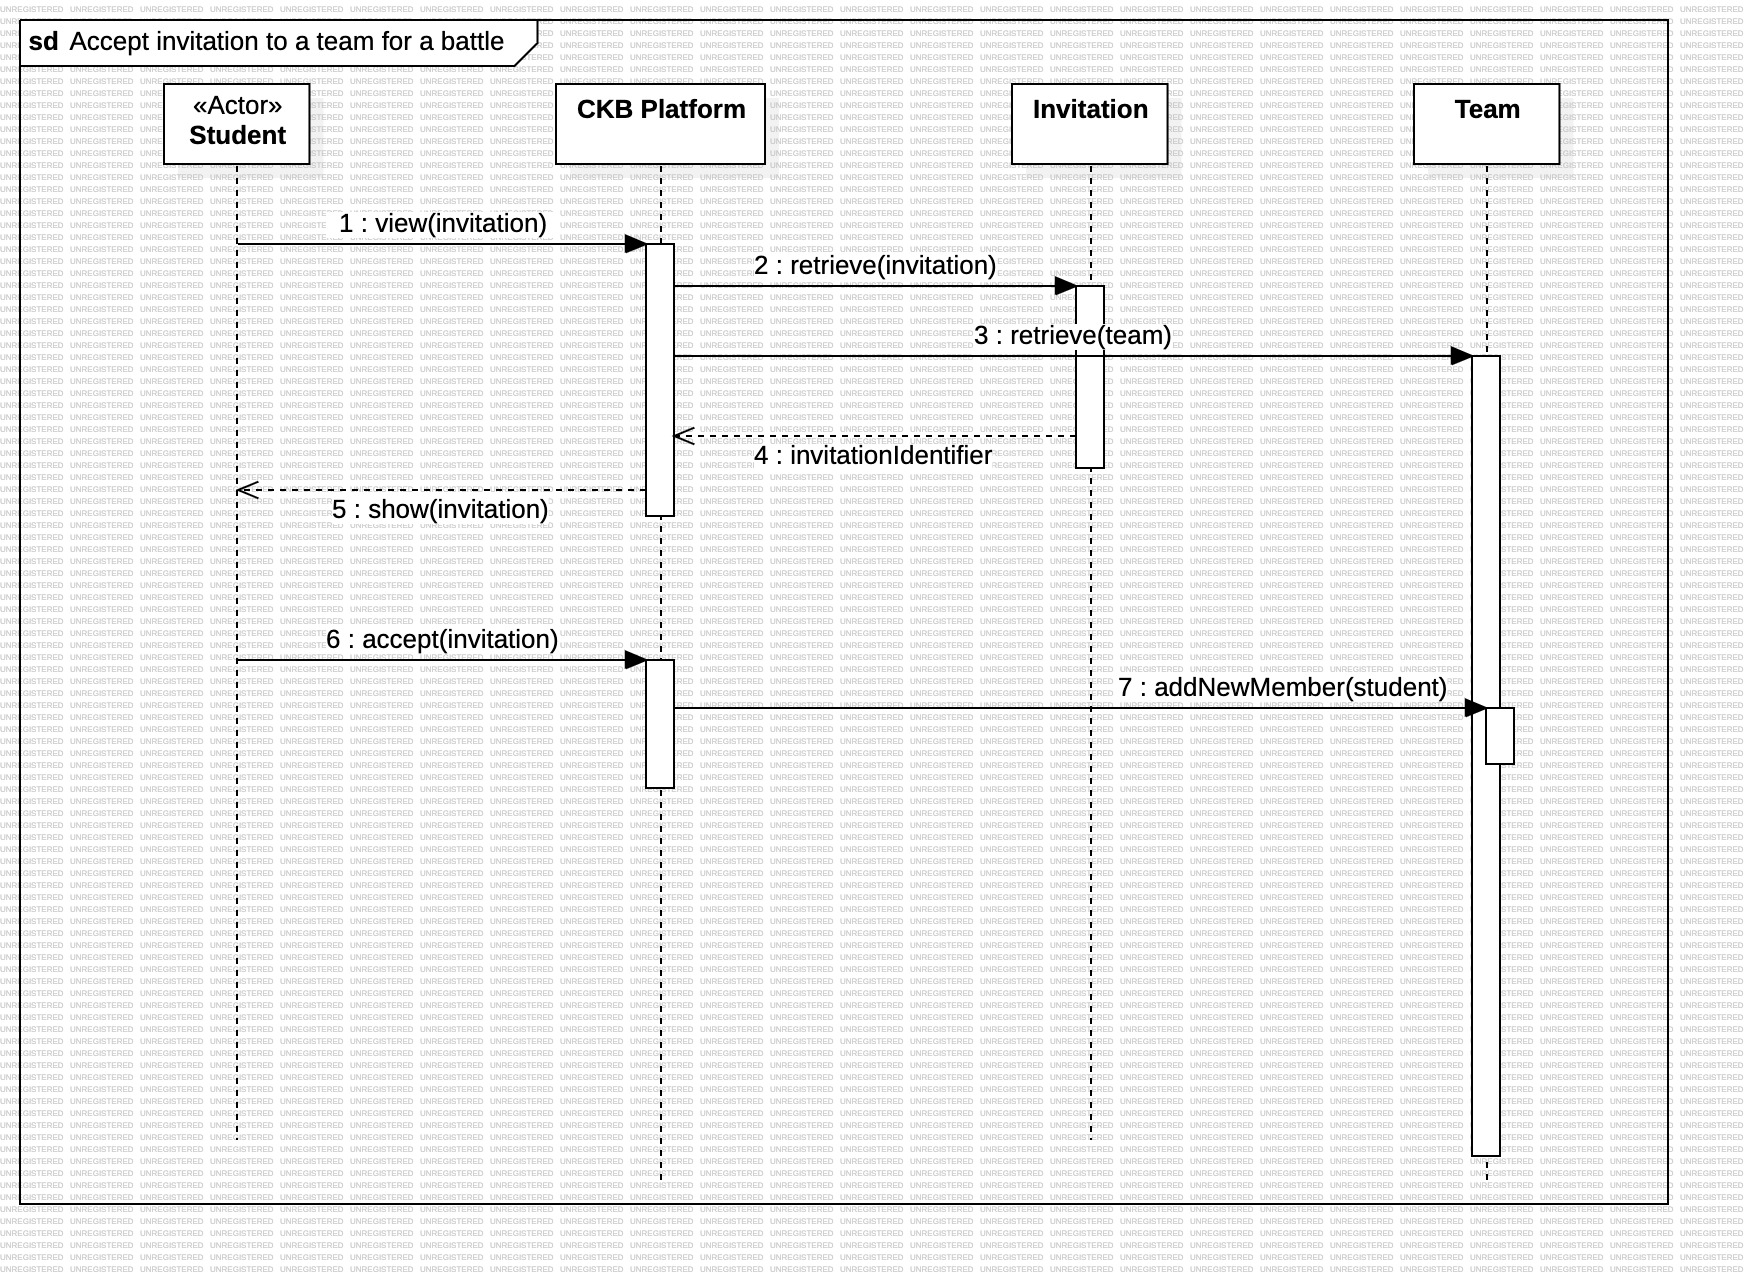
\includegraphics[width=\textwidth]{Diagrams/StudentAcceptInvitation.jpg}
    \caption{Sequence Diagram - Accept invitation to a team for a battle}
    \label{fig:sequence-diagram-accept-invitation}
\end{figure}
\subsubsection*{[UC13] Invite other students to the team}
\begin{figure}[H]
    \centering
    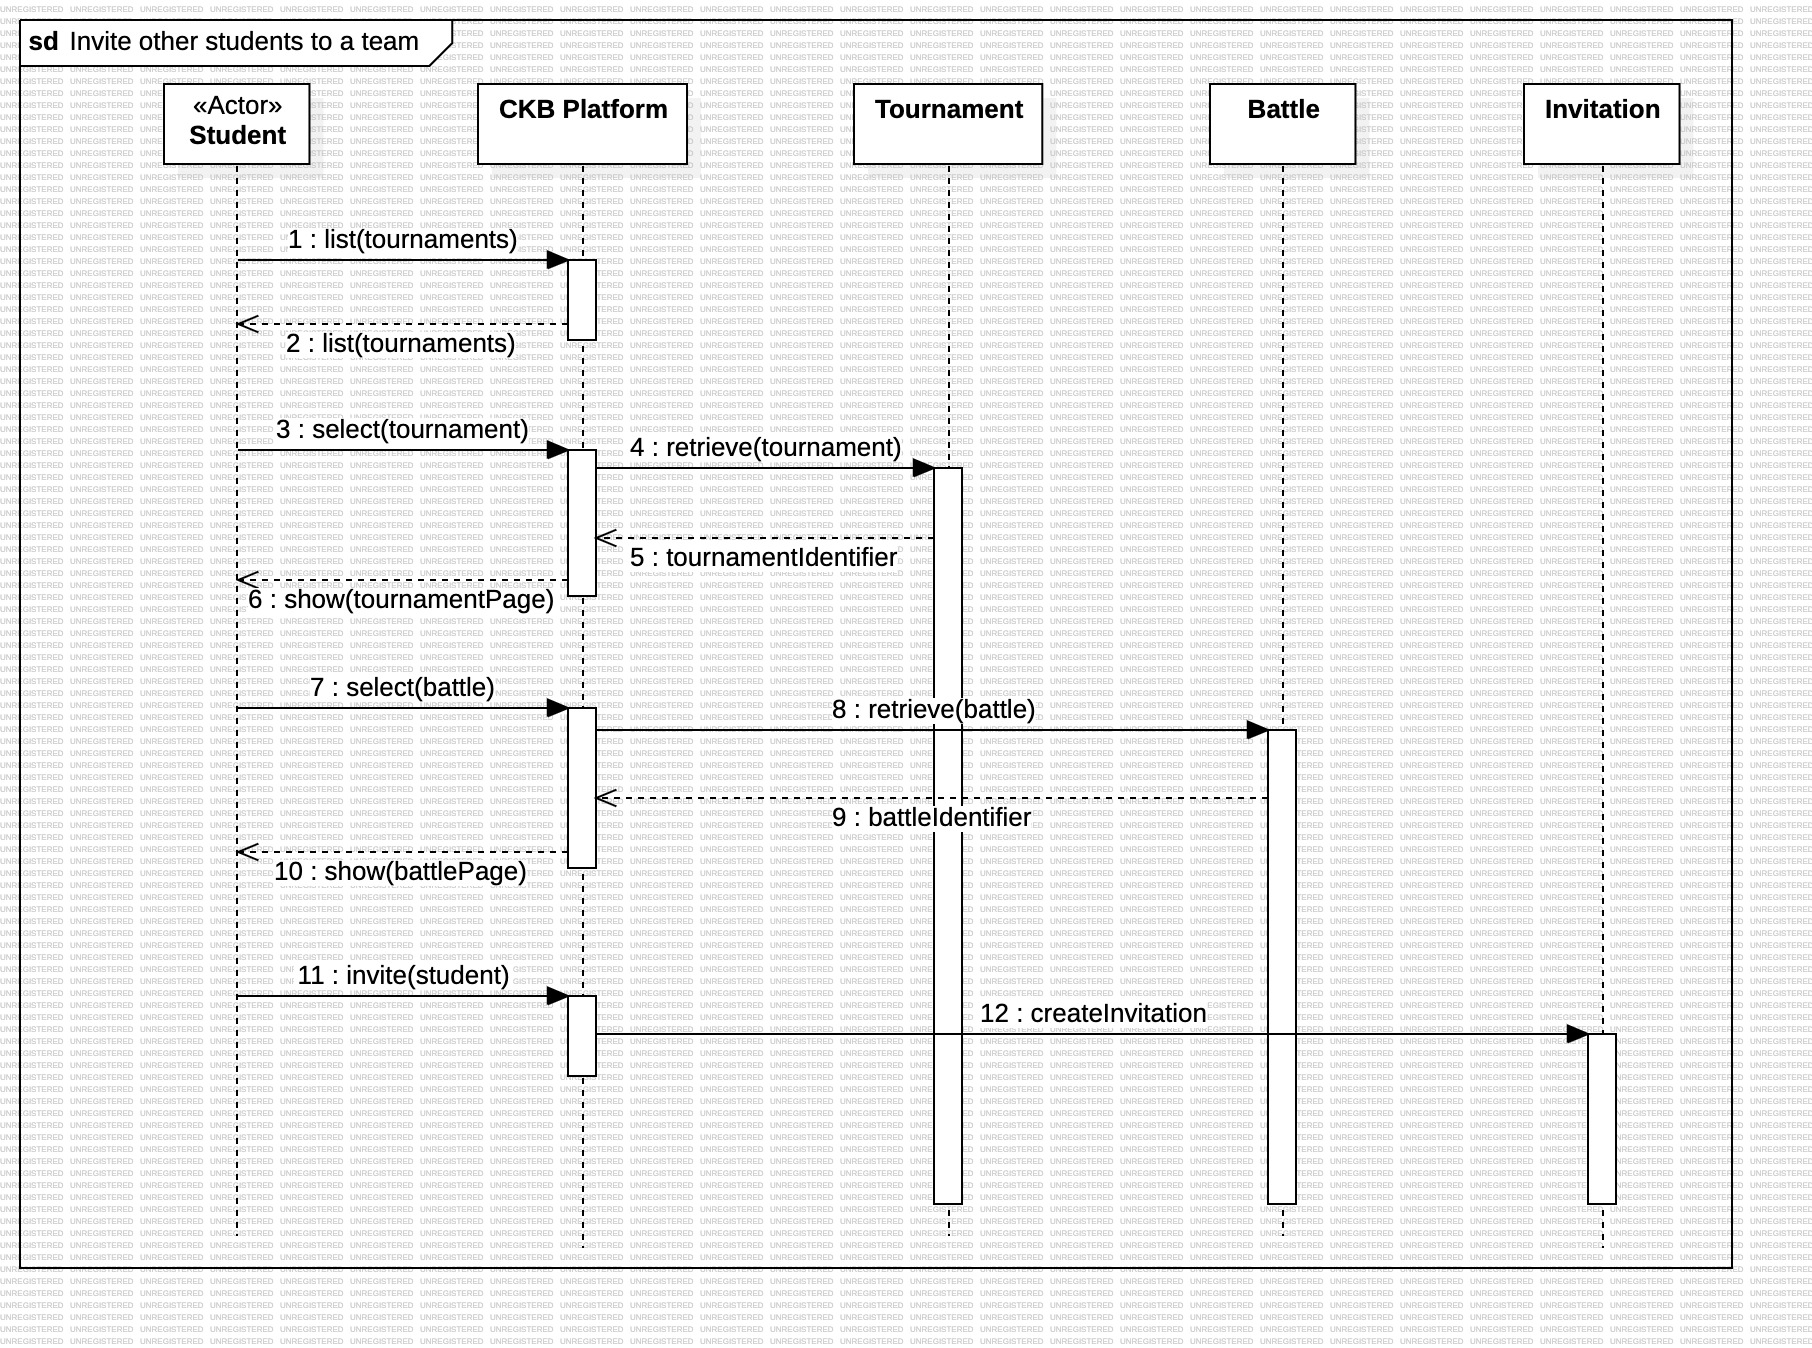
\includegraphics[width=\textwidth]{Diagrams/StudentInvitation.jpg}
    \caption{Sequence Diagram - Invite other students to the team}
    \label{fig:sequence-diagram-invite-students}
\end{figure}
\subsubsection*{[UC15] Submission of a solution for a battle}
\begin{figure}[H]
    \centering
    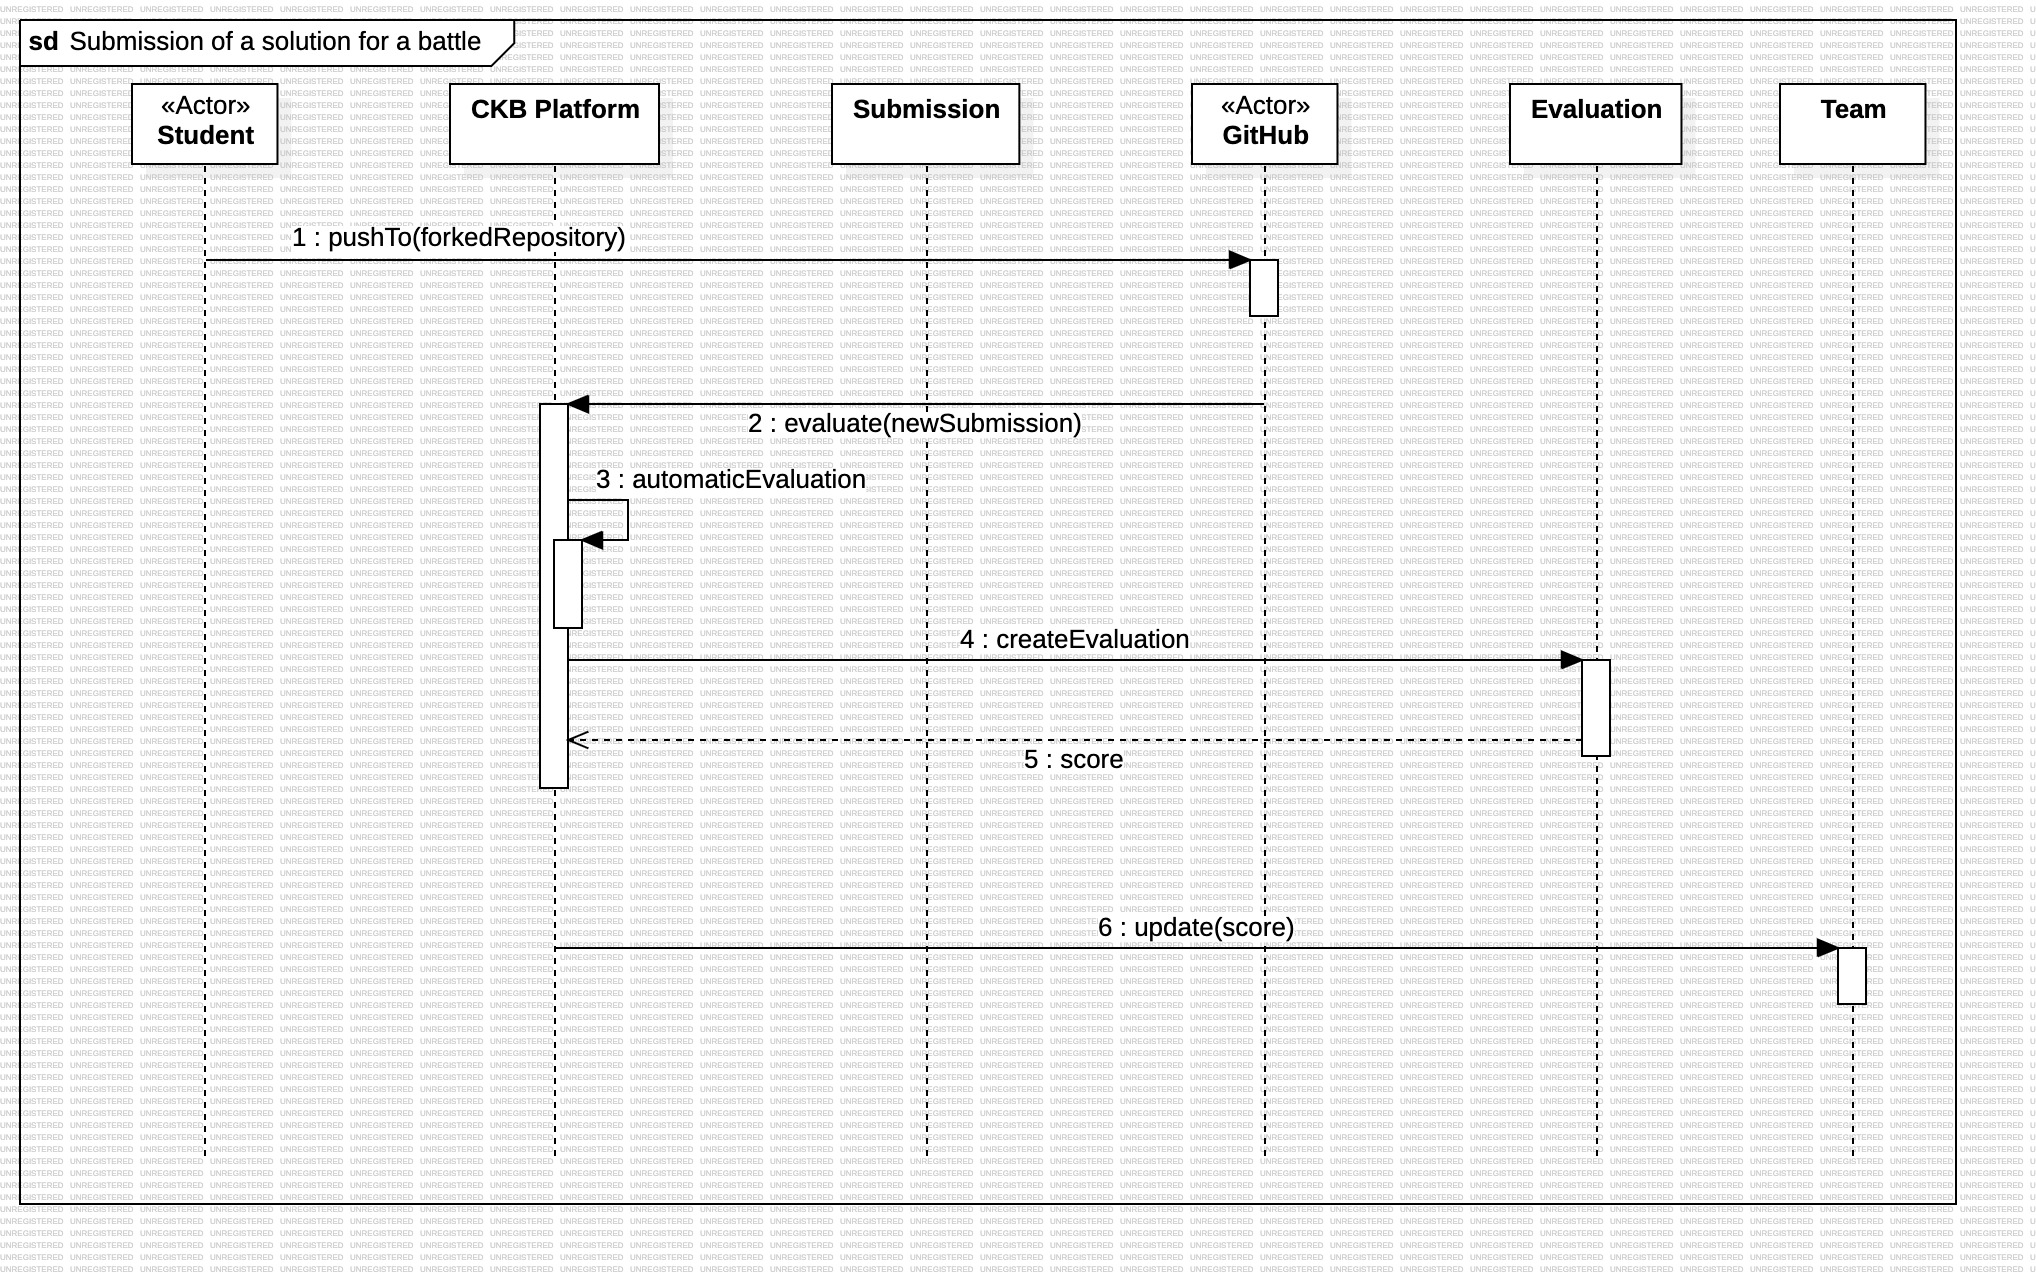
\includegraphics[width=\textwidth]{Diagrams/Submission.jpg}
    \caption{Sequence Diagram - Submission of a solution for a battle}
    \label{fig:sequence-diagram-submission}
\end{figure}
\subsubsection*{[UC17] Automatic evaluation of a submission}
\begin{figure}[H]
    \centering
    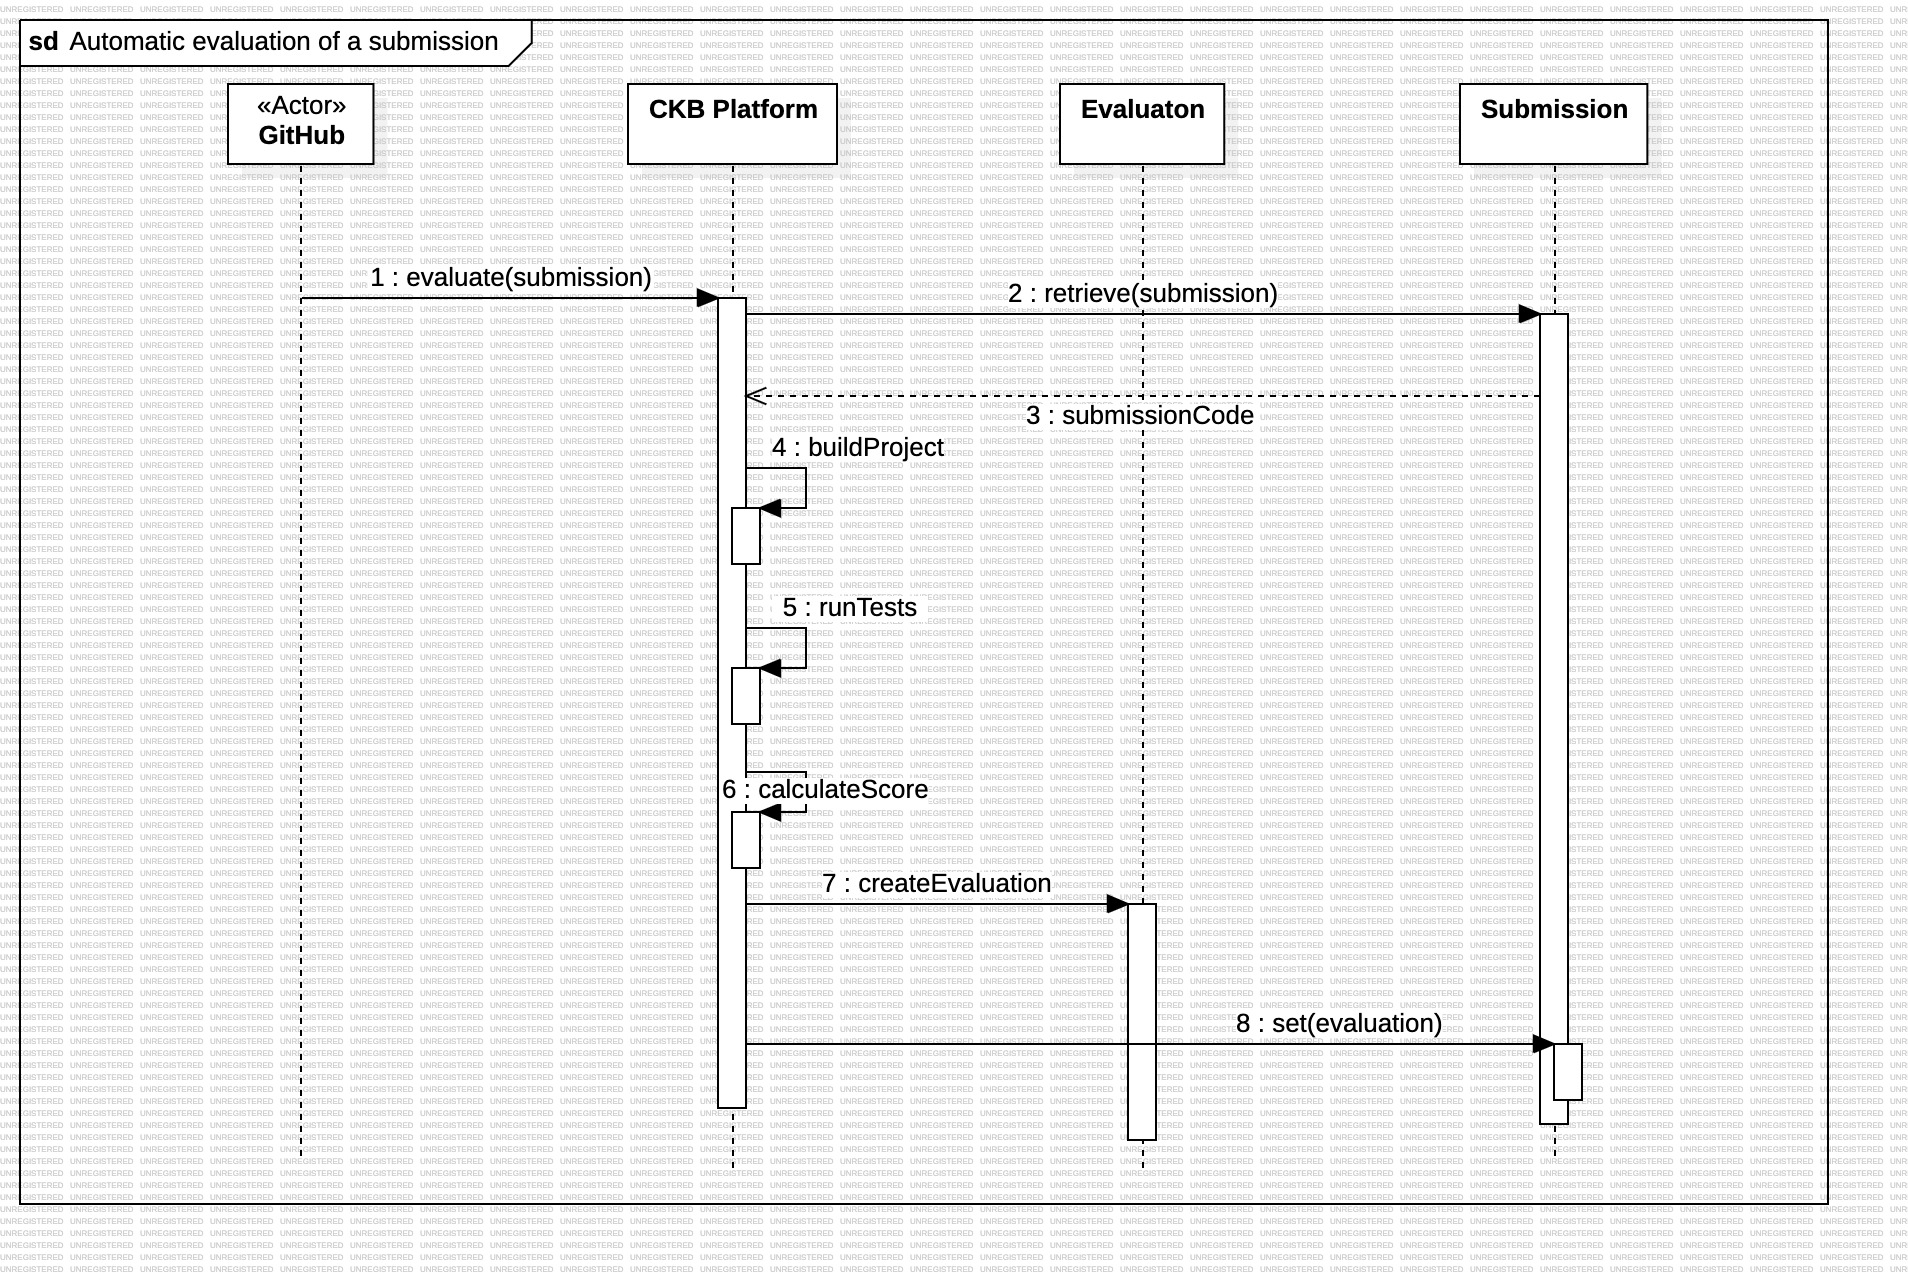
\includegraphics[width=\textwidth]{Diagrams/AutomaticEvaluation.jpg}
    \caption{Sequence Diagram - Automatic evaluation of a submission}
    \label{fig:sequence-diagram-automatic-evaluation}
\end{figure}
\subsubsection*{[UC1] Login}
\begin{figure}[H]
    \centering
    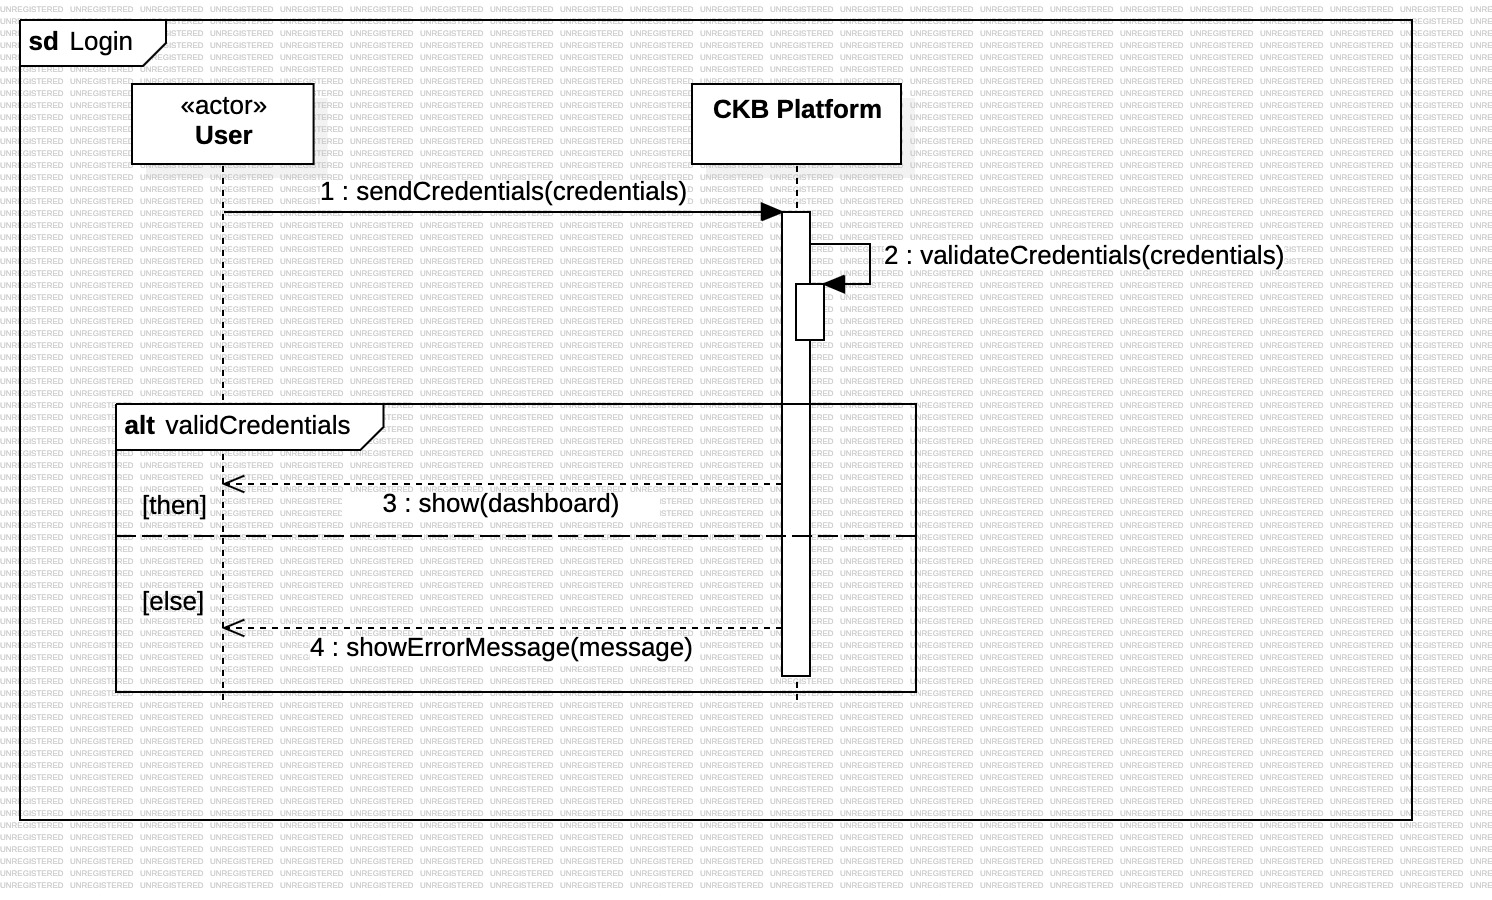
\includegraphics[width=\textwidth]{Diagrams/UC1SequenceDiagram.jpg}
    \caption{Sequence Diagram for the Login Use Case}
    \label{fig:sequence-diagram-login}
\end{figure}

\subsubsection*{[UC3] Close a tournament}
\begin{figure}[H]
    \centering
    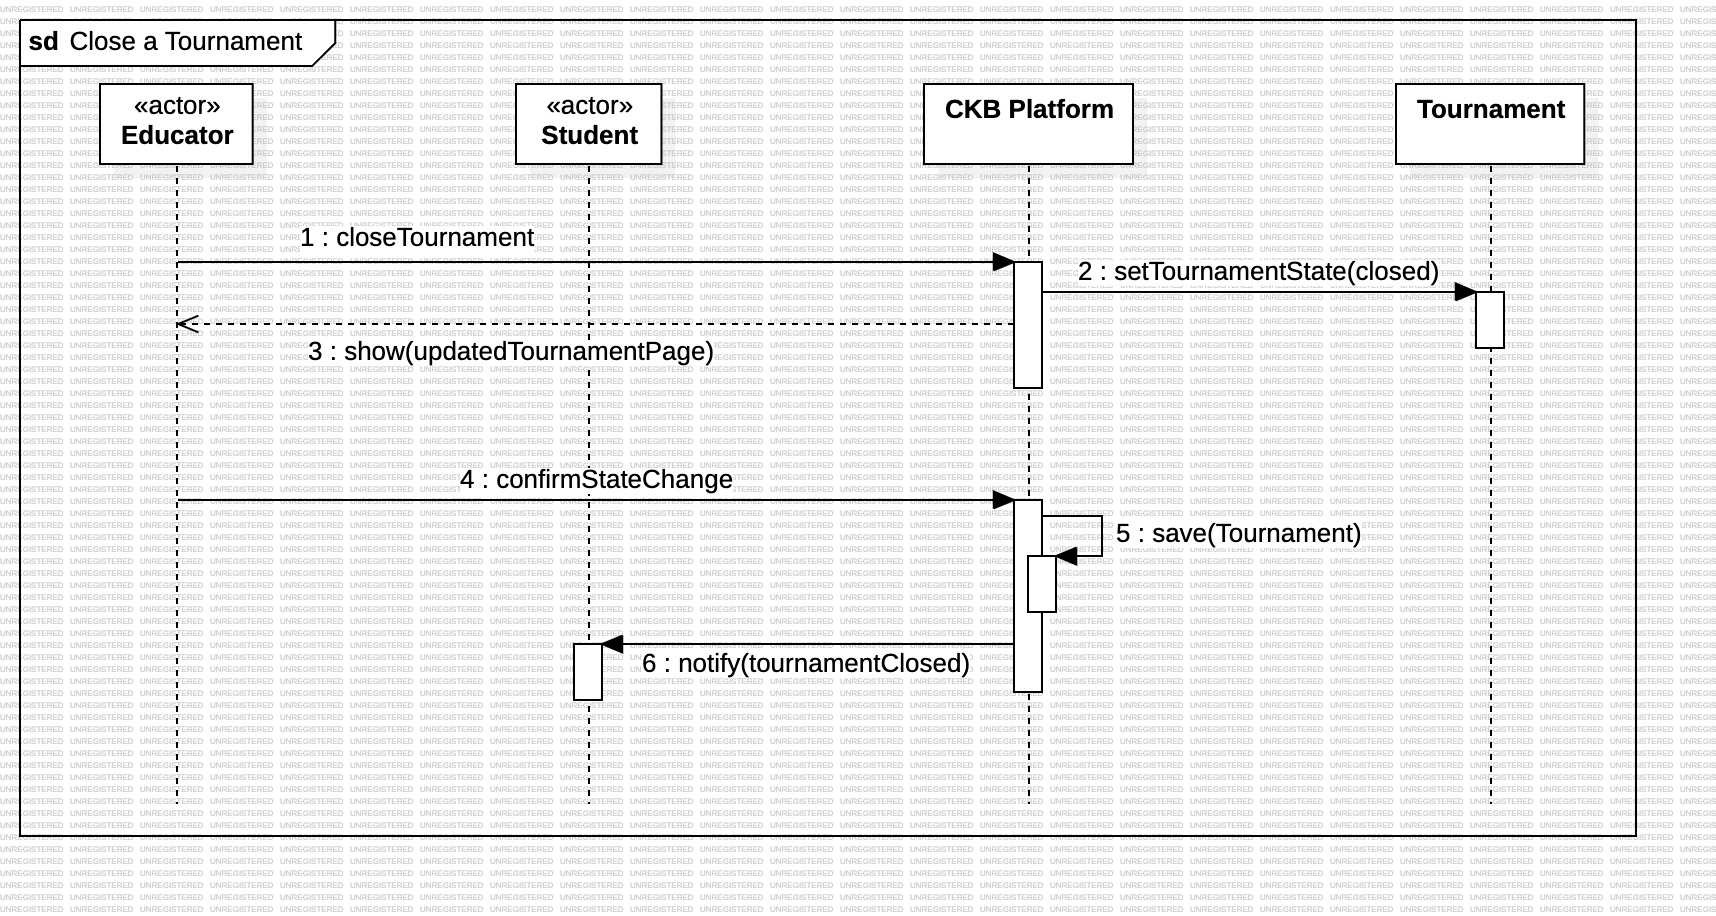
\includegraphics[width=\textwidth]{Diagrams/UC3SequenceDiagram.jpg}
    \caption{Sequence Diagram for the Close a tournament Use Case}
    \label{fig:sequence-diagram-close-tournament}
\end{figure}

\subsubsection*{[UC5] Upload of code kata}
\begin{figure}[H]
    \centering
    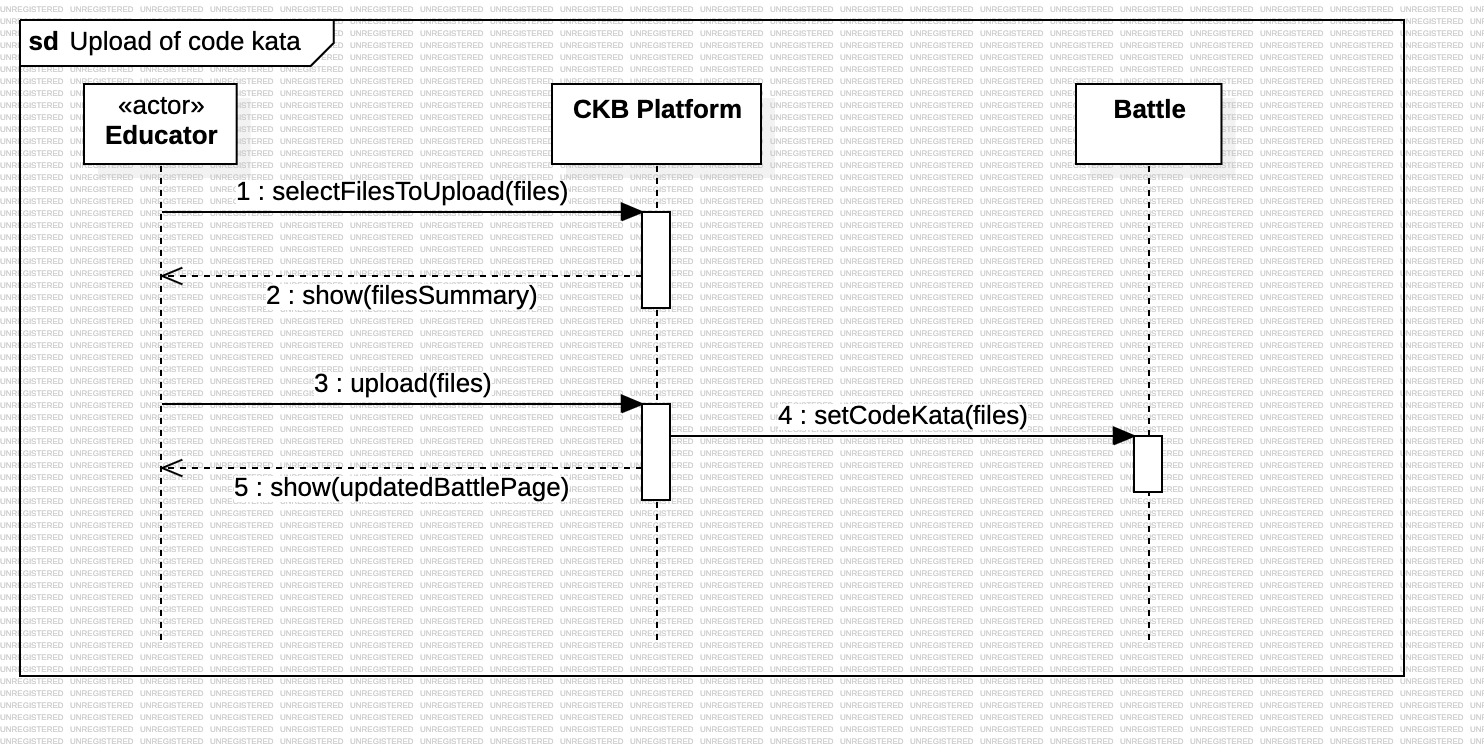
\includegraphics[width=\textwidth]{Diagrams/UC5SequenceDiagram.jpg}
    \caption{Sequence Diagram for the Upload of code kata Use Case}
    \label{fig:sequence-diagram-upload-code-kata}
\end{figure}

\subsubsection*{[UC6] Manual score update}
\begin{figure}[H]
    \centering
    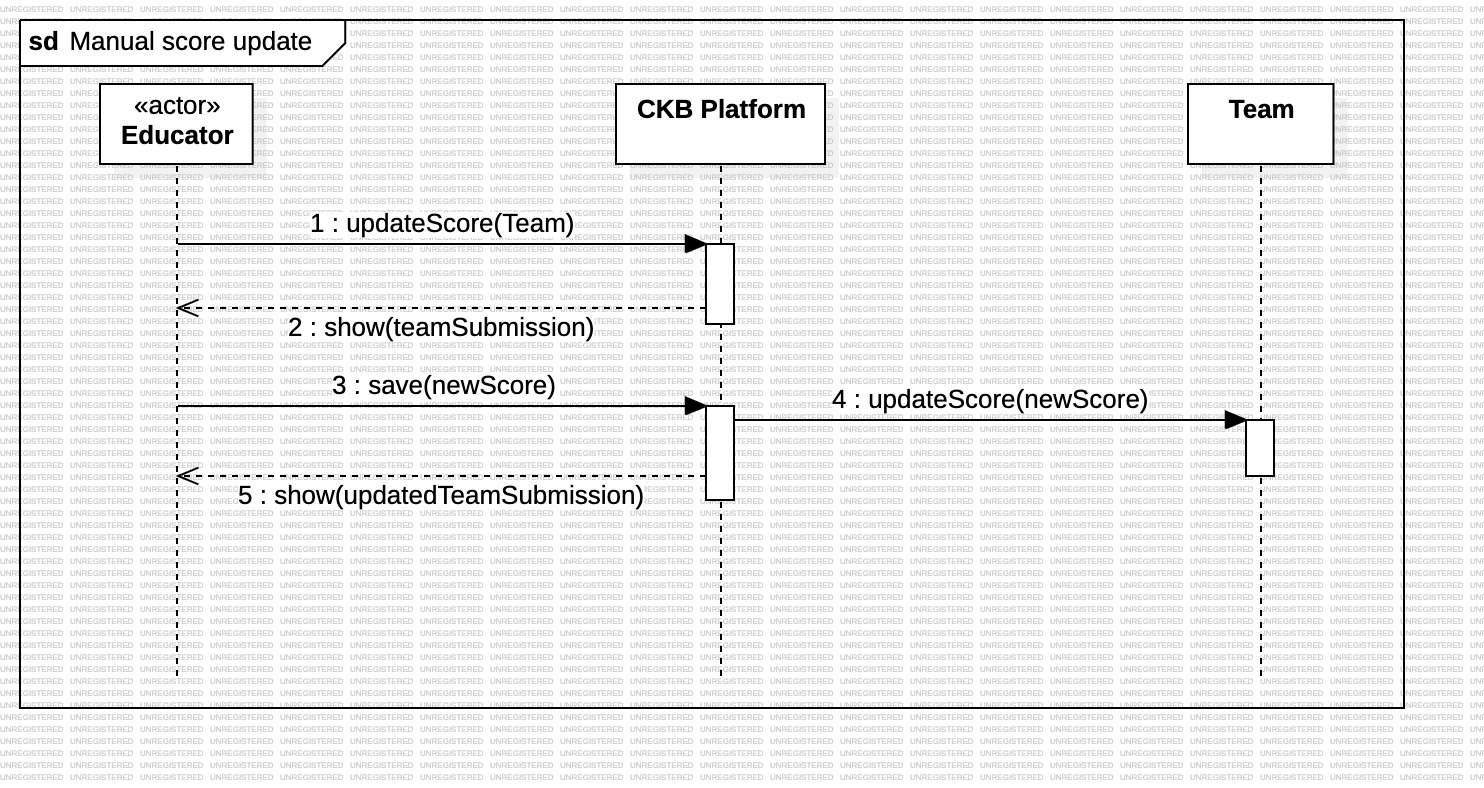
\includegraphics[width=\textwidth]{Diagrams/UC6SequenceDiagram.jpg}
    \caption{Sequence Diagram for the Manual score update Use Case}
    \label{fig:sequence-diagram-manual-score-update}
\end{figure}

\subsubsection*{[UC8] Notification to a student}
\begin{figure}[H]
    \centering
    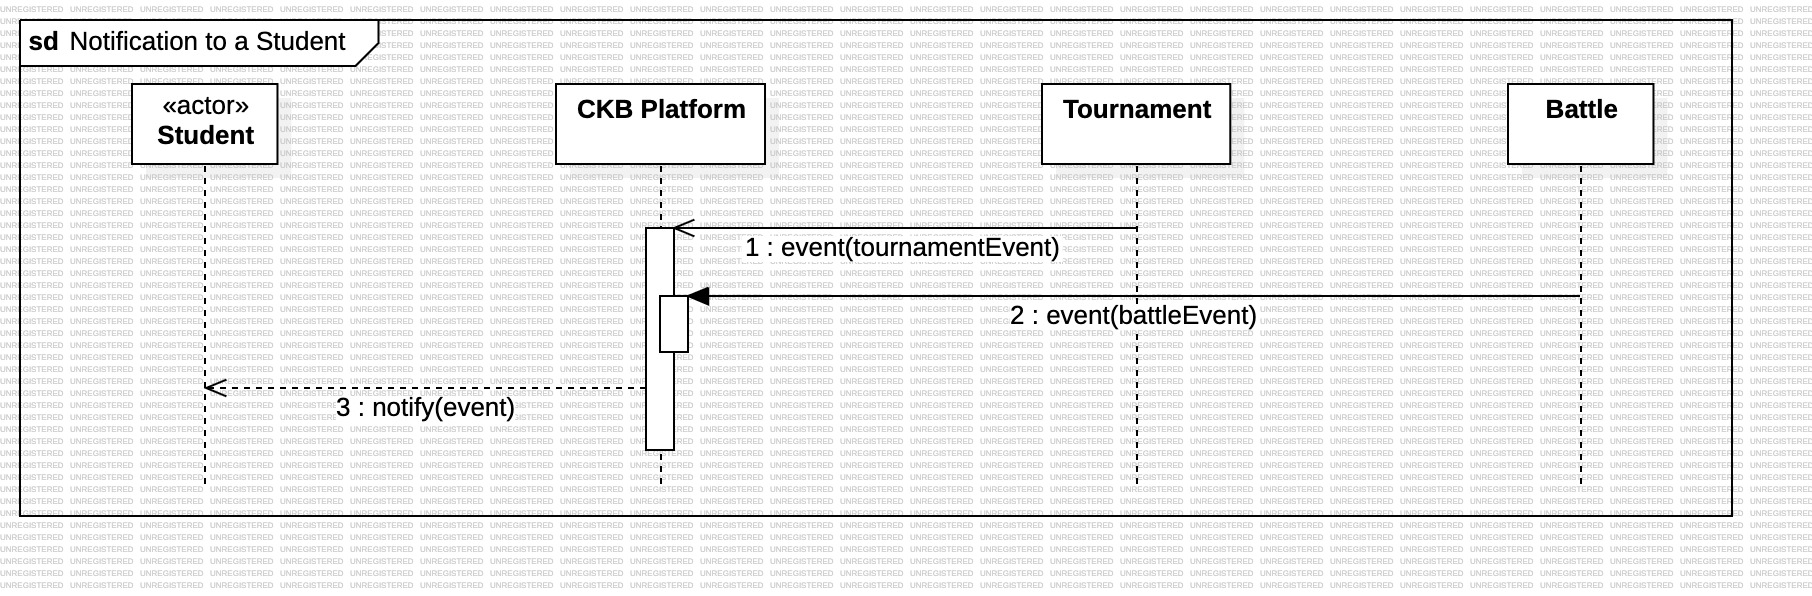
\includegraphics[width=\textwidth]{Diagrams/UC8SequenceDiagram.jpg}
    \caption{Sequence Diagram for the Notification to a student Use Case}
    \label{fig:sequence-diagram-notification}
\end{figure}

\subsubsection*{[UC10] Subscribe to a battle}
\begin{figure}[H]
    \centering
    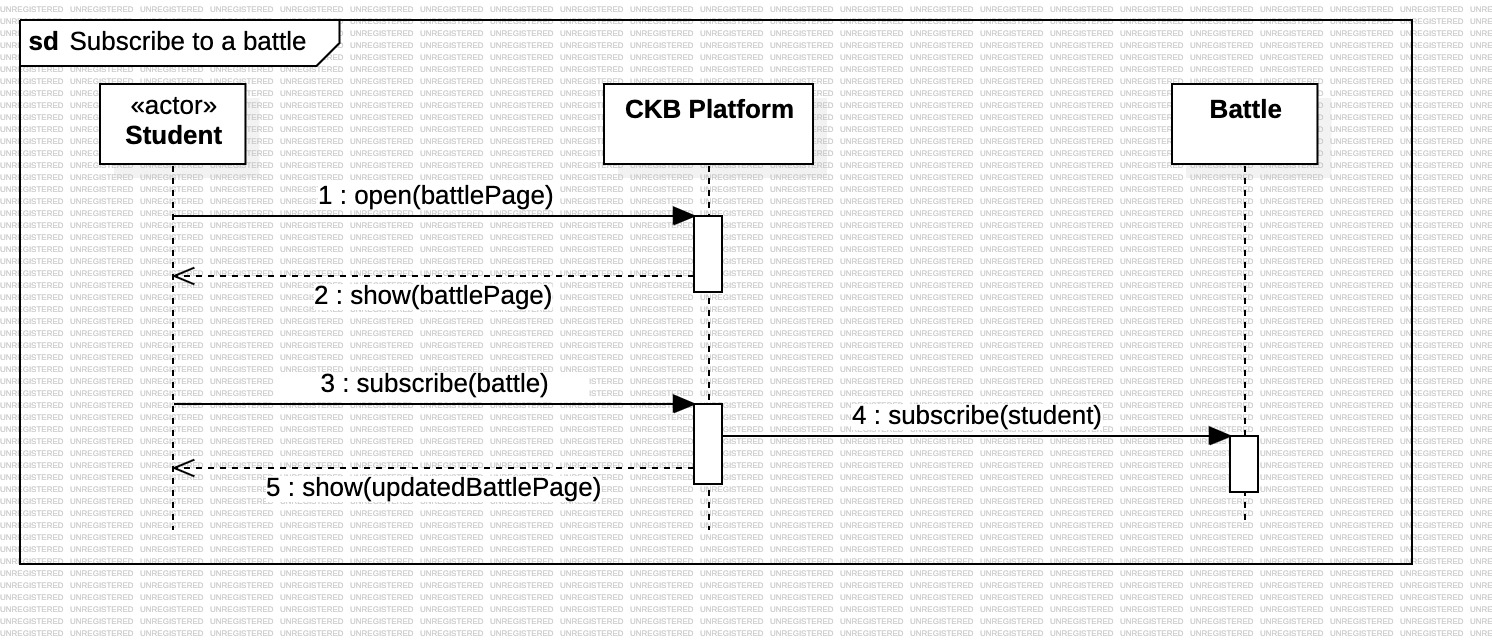
\includegraphics[width=\textwidth]{Diagrams/UC10SequenceDiagram.jpg}
    \caption{Sequence Diagram for the Subscribe to a battle Use Case}
    \label{fig:sequence-diagram-subscribe-battle}
\end{figure}

\subsubsection*{[UC12] Creation of a team for a battle}
\begin{figure}[H]
    \centering
    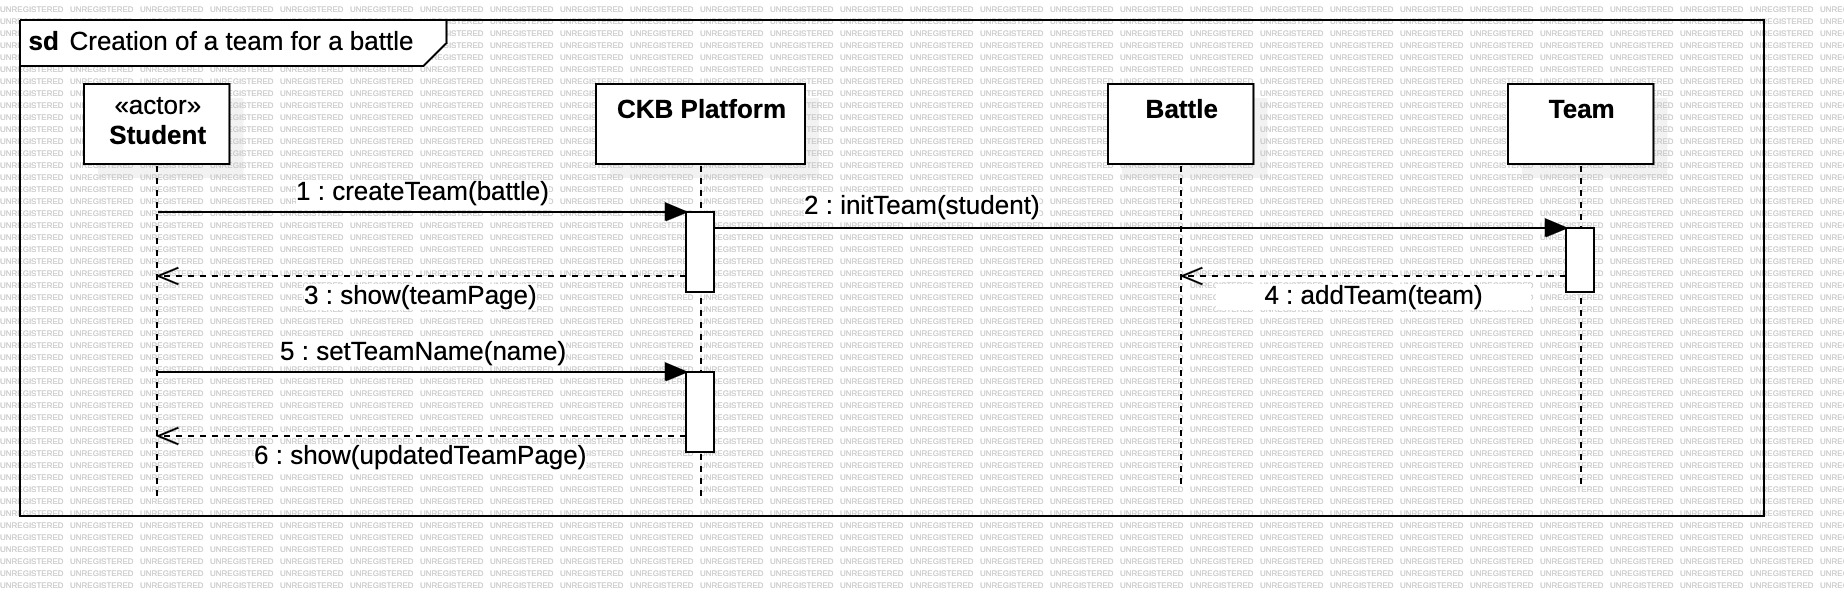
\includegraphics[width=\textwidth]{Diagrams/UC12SequenceDiagram.jpg}
    \caption{Sequence Diagram for the Creation of a team for a battle Use Case}
    \label{fig:sequence-diagram-create-team}
\end{figure}

\subsubsection*{[UC14] Fork repository of a battle}
\begin{figure}[H]
    \centering
    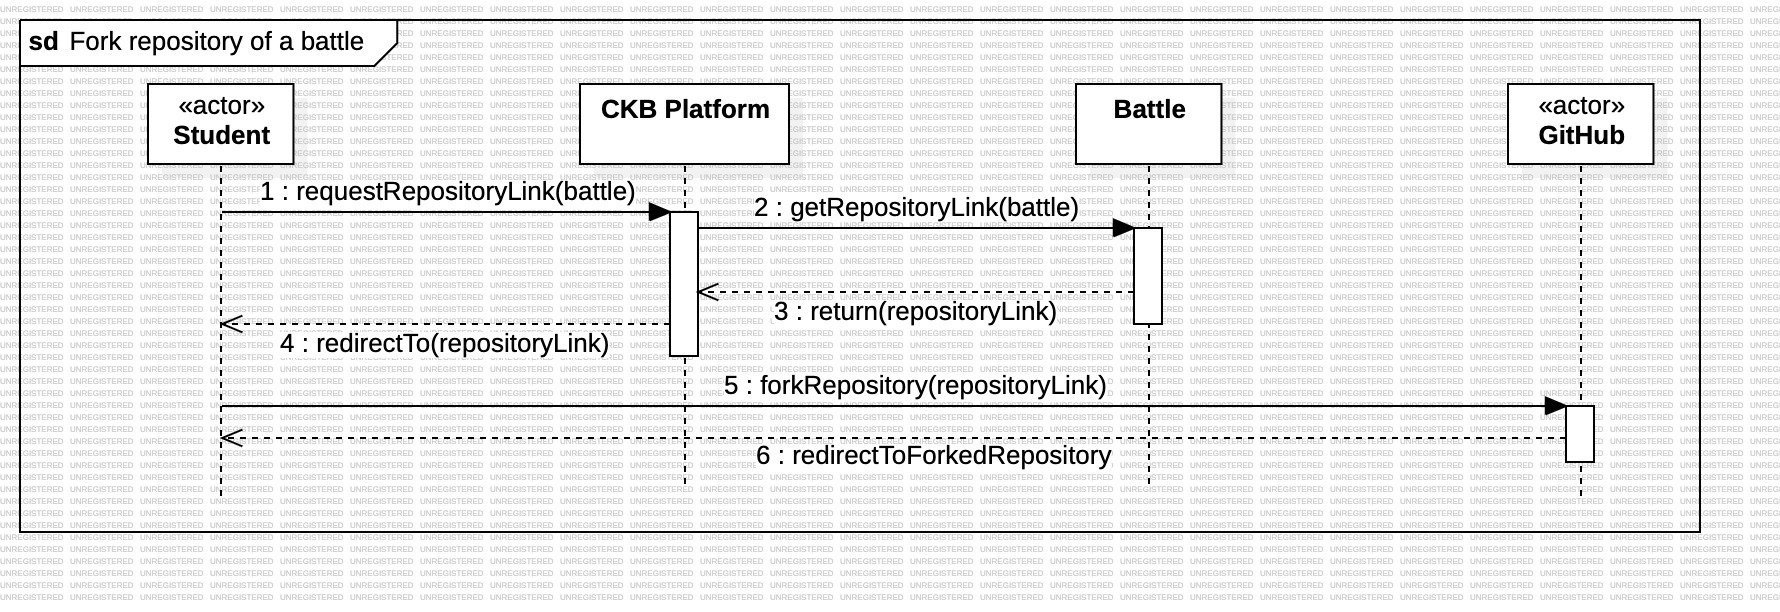
\includegraphics[width=\textwidth]{Diagrams/UC14SequenceDiagram.jpg}
    \caption{Sequence Diagram for the Fork repository of a battle Use Case}
    \label{fig:sequence-diagram-fork-repository}
\end{figure}

\subsubsection*{[UC16] Push on team repository}
\begin{figure}[H]
    \centering
    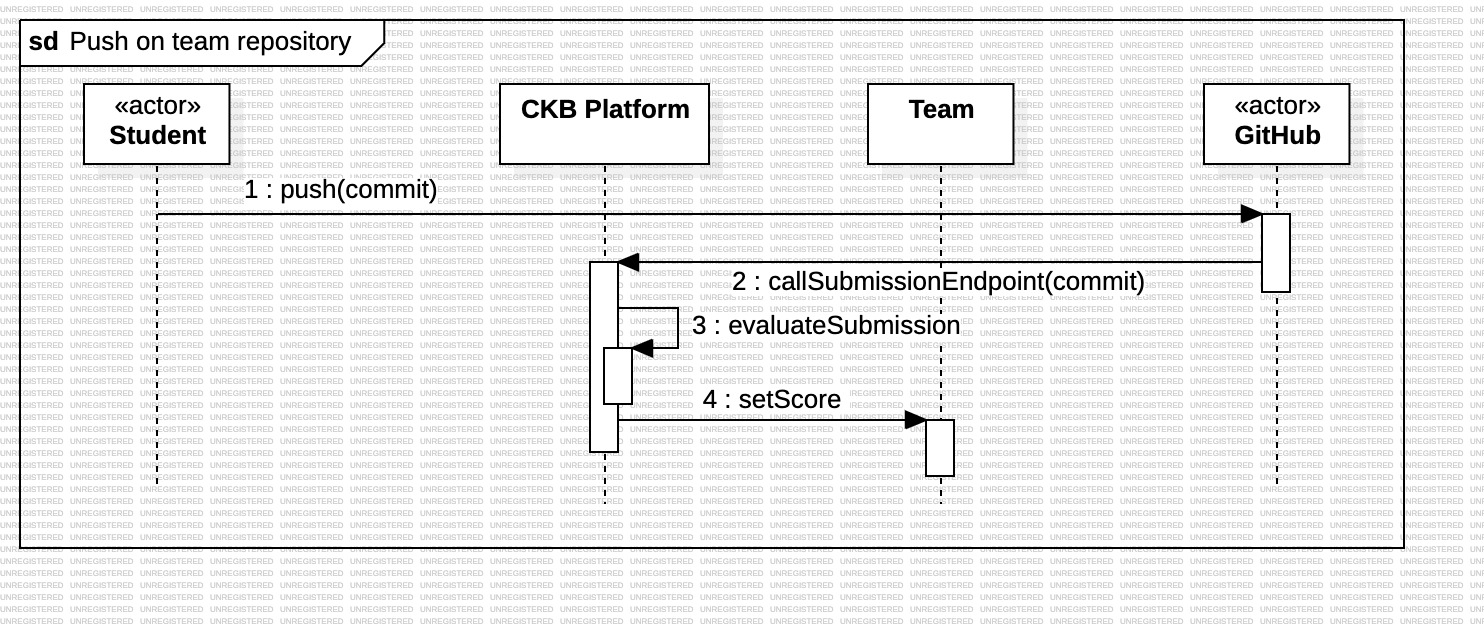
\includegraphics[width=\textwidth]{Diagrams/UC16SequenceDiagram.jpg}
    \caption{Sequence Diagram for the Push on team repository Use Case}
    \label{fig:sequence-diagram-push-repository}
\end{figure}



\subsubsection{Requirements mapping}
\begin{tabular}{|p{6cm}|p{6cm}|}
    \hline
    \multicolumn{2}{|c|}{[G1] Educator can create a torunament} \\
    \hline
    \begin{itemize}
        \item [R1]
        \item [R2]
        \item [R3]
    \end{itemize}
    &
    \begin{itemize}
        \item [D1]
        \item [D3]
    \end{itemize}
    \\
    \hline
\end{tabular}

\begin{tabular}{|p{6cm}|p{6cm}|}
    \hline
    \multicolumn{2}{|c|}{[G2] Educator can setup battles for a tournament} \\
    \hline
    \begin{itemize}
        \item [R1]
        \item [R2]
        \item [R4]
        \item [R5]
        \item [R6]
    \end{itemize}
    &
    \begin{itemize}
        \item [D1]
        \item [D3]
    \end{itemize}
    \\
    \hline
\end{tabular}

\begin{tabular}{|p{6cm}|p{6cm}|}
    \hline
    \multicolumn{2}{|c|}{[G3] Student can partecipate in a tournament} \\
    \hline
    \begin{itemize}
        \item [R1]
        \item [R2]
        \item [R7]
        \item [R8]
    \end{itemize}
    &
    \begin{itemize}
        \item [D1]
        \item [D2]
        \item [D3]
    \end{itemize}
    \\
    \hline
\end{tabular}

\begin{tabular}{|p{6cm}|p{6cm}|}
    \hline
    \multicolumn{2}{|c|}{[G4] Team of students can submit a solution for a battle} \\
    \hline
    \begin{itemize}
        \item [R1]
        \item [R2]
        \item [R7]
        \item [R8]
        \item [R9]
    \end{itemize}
    &
    \begin{itemize}
        \item [D1]
        \item [D2]
        \item [D3]
        \item [D4]
        \item [D8å]
    \end{itemize}
    \\
    \hline
\end{tabular}

\begin{tabular}{|p{6cm}|p{6cm}|}
    \hline
    \multicolumn{2}{|c|}{[G5] Educator can manually update the score of a team in a battle} \\
    \hline
    \begin{itemize}
        \item [R1]
        \item [R2]
        \item [R19]
    \end{itemize}
    &
    \begin{itemize}
        \item [D1]
        \item [D3]
        \item [D4]
        \item [D8]
        \item [D9]
    \end{itemize}
    \\
    \hline
\end{tabular}

\begin{tabular}{|p{6cm}|p{6cm}|}
    \hline
    \multicolumn{2}{|c|}{[G6] CKB notify the student about upcoming tournaments} \\
    \hline
    \begin{itemize}
        \item [R1]
        \item [R12]
    \end{itemize}
    &
    \begin{itemize}
        \item [D1]
        \item [D3]
        \item [D6]
    \end{itemize}
    \\
    \hline
\end{tabular}

\begin{tabular}{|p{6cm}|p{6cm}|}
    \hline
    \multicolumn{2}{|c|}{[G7] CKB notify the student about upcoming battles} \\
    \hline
    \begin{itemize}
        \item [R1]
        \item [R13]
    \end{itemize}
    &
    \begin{itemize}
        \item [D1]
        \item [D3]
        \item [D7]
    \end{itemize}
    \\
    \hline
\end{tabular}
